\documentclass[a4paper]{article}
\usepackage[utf8]{inputenc}
\usepackage{amsthm}
\usepackage{amsfonts}
\usepackage{amssymb}
\usepackage{amsmath}
\usepackage{tikz}
\usepackage{pgfplots}
\usepackage{esint}
\usepackage{geometry}

\usepgfplotslibrary{fillbetween}

\setlength\parskip{0.3em}
\setlength{\parindent}{0 pt}

\theoremstyle{definition}

\newcommand{\Ker}{\text{Ker}}
\newcommand{\curl}{\text{curl }}

\newtheorem{defn}{Definition}[subsection]
\newtheorem{prop}[defn]{Proposition}
\newtheorem{thm}[defn]{Theorem}
\newtheorem{lemma}[defn]{Lemma}
\newtheorem{coro}[defn]{Corollary}
\newtheorem{eg}[defn]{Example}
\newtheorem*{remark}{Remark}
\newtheorem*{notation}{Notation}

\title{MA259 Multivariable calculus :: Lecture notes}
\author{Lecturer: Mario Micallef}
\date{\today}

\begin{document}

\maketitle
\thispagestyle{empty}

\tableofcontents
\thispagestyle{empty}
\newpage
\setcounter{page}{1}

Topics
\begin{itemize}
	\item Continuity and differentiability of $f: \mathbb{R}^n \rightarrow \mathbb{R}^k$
	\item Higher dimensional version of FTC
\end{itemize}

Difference between column and row vectors.

\begin{itemize}
	\item Column vector $v=\begin{pmatrix}
		v_1 \\ \vdots \\ v_n
	\end{pmatrix}$ represents linear map $T: \mathbb{R} \rightarrow \mathbb{R}^n$, $T(t) = tv$ (line through 0 in dir $v$)
	\item Row vector $v=(v_1,\ldots,v_n)$ represents $\lambda_v:\mathbb{R}^n \rightarrow \mathbb{R}$, $\lambda_v(x)=v_1x_1+\cdots+v_nx_n$ (linear functional)
	\begin{itemize}
		\item Ker $\lambda_v = \{ x \in \mathbb{R}^n, \lambda_v(x)=0, \text{i.e. }v^T \cdot x =0 \}=H_v$, hyperplane $\perp v^T$ through 0
		\item Level set $\Gamma_c=\{ x \in \mathbb{R}^n : \lambda_v(x)=c, \text{i.e. } v^T \cdot x=c \}$ ($c\in \mathbb{R}$)
	\end{itemize} 
\end{itemize}

\section{Convergence of a sequence}
Recall the definition of convergence from Analysis I.
\begin{defn}
	$x_j$ is a sequence of vectors $\in \mathbb{R}^n$. We say $x_j \rightarrow x$ if $\forall \varepsilon > 0,$ $\exists N \in \mathbb N$ such that $j \geq N \Rightarrow \underbrace{|x_j-x|}_{\text{Euclidean distance=}\sqrt{(x_1-x_{1j})^2+\cdots +(x_n-x_{nj})^2}} < \varepsilon$.
\end{defn}

\begin{prop}
	Limit is unique.
\end{prop}

\begin{prop}
	[componentwise convergence] A sequence $x_j=(x_{1j} \ldots x_{nj})$ converges to $x=(x_1 \ldots x_n)$ if and only if $\forall i$, $x_{ij} \rightarrow x_i$ .
\end{prop}
\begin{proof}
	``$\Rightarrow$'' Suppose $x_j \rightarrow x$. Observe, $\forall i$, $|x_{ij}-x_i| \leq \sqrt{\sum_i (x_{ij}-x_i)^2}=|x_j-x| \rightarrow 0$. By sandwich $|x_{ij}-x_i| \rightarrow 0$ so $x_{ij} \rightarrow x_i$.

	``$\Leftarrow$'' Suppose $\forall i$, $x_{ij}\rightarrow x_i$. Then given $\varepsilon > 0$, $\exists N_i \in \mathbb N$ such that $j \geq N_i \Rightarrow |x_{ij}-x_i|<\varepsilon$. Set $N=\max \{N_i\}$. Then
\[
|x_j-x| \leq \sqrt{n\varepsilon^2}=\sqrt n \varepsilon \quad \Rightarrow \quad x_j \rightarrow x .
\]
\end{proof}
\begin{remark}
	That ``$\max \{\}$'' can be seen as a norm:
	\begin{itemize}
		\item $|x|_{\infty} := \max \{ |x_1|,|x_2|,\ldots |x_n| \}$
		\item NY taxi cab norm: $|x|_1 := |x_1|+\cdots +|x_n|$
		\item more generally, $|x|_p := \left( |x_1|^p + \cdots |x_n|^p \right)^{1/p}$ 
	\end{itemize}
\end{remark}
\begin{remark}
	The theorem above in Euclidean norm is equivalent to that in $|.|_{\infty}$.
\end{remark}

\begin{lemma}
	If $x_j \rightarrow x$ then $|x_j| \rightarrow |x|$.
\end{lemma}
\begin{proof}
	Given $\varepsilon >0$, $\exists N \in \mathbb N$ such that $j \geq N \Rightarrow |x_j-x|<\varepsilon \Rightarrow ||x_j|-|x|| \leq |x_j-x| < \varepsilon$.
\end{proof}
\begin{remark}
	$|x_j|$ converges $\not\Rightarrow$ $x_j$ converges.
\end{remark}

\section{Continuity}
\begin{defn} [$\varepsilon-\delta$]
	$f:U\rightarrow \mathbb R^k$ where $U \subset \mathbb R ^n$ is continuous at $p\in U$ if $\forall \varepsilon >0$, $\exists \delta >0$ such that $|x-p|<\delta \Rightarrow |f(x)-f(p)| < \varepsilon$ and $x\in U$.
\end{defn}
\begin{defn} [sequential]
	$f:U\rightarrow \mathbb R^k$ is continous at $p$ if $\forall x_j \rightarrow p$, $f(x_j) \rightarrow f(p)$.
\end{defn}
\begin{notation}
	$\mathcal C (U, \mathbb R^k) = \{ f: U \rightarrow \mathbb R^k, f\text{ is continuous at all points of }U \}$
\end{notation}
\begin{defn}
	$f:U\rightarrow \mathbb R^k$ has a limit at $p\in U$ if $\exists q \in \mathbb R^k$ such that $\forall \varepsilon >0$, $\exists \delta >0 : 0<|x-p|<\delta \Rightarrow |f(x)-q|<\varepsilon$. Then we write
\[
\lim_{x\rightarrow p} f(x)=q.
\]
\end{defn}
\subsection{Separate continuity}
How do transport what we know about 1-d functions in Analysis to multivariable ones? Vertical slicing of $f: \mathbb R^2 \rightarrow \mathbb R$. (seen in MA134 when introducing partial derivative)

Given $f: \mathbb R^2 \rightarrow \mathbb R$ then for each fixed $y \in \mathbb R$ we consider $g^y : \mathbb R \rightarrow \mathbb R$ defined by $g^y(x) := f(x,y)$, which is a familiar function of one variable.

\begin{eg}
	$f(x,y)=x \sin y.$ Then $g^1(x) = (\sin 1) x$. We then see $f$ as a family of one-real-variable linear functions, with the parameter $y$ varying them around the origin.
\end{eg}

Similarly for each $x\in \mathbb R$ we consider $h^x : \mathbb R \rightarrow \mathbb R$ defined by $h^x(y) := f(x,y).$

\begin{eg}
	Using the same $f$ above, this is now a family of sine curves with $x$ as a parameter (amplitude), e.g. $h^3(y)=3\sin y.$
\end{eg}

The graphs (curves) of $g^s$ and $h^t$ are obtained by intersecting the graph of $f$ (a surface) with the vertical plane $y=s$ and $x=t$ respectively. (vertical slicing of the graph of $f$.)

\begin{defn} [separate continuity]
	$f:\mathbb R^2 \rightarrow \mathbb R$ is separately continuous at $(x_0,y_0)$ if $g^{y_0}$ is continuous at $x_0$ and $h^{x_0}$ is continuous at $y_0$.
\end{defn}

\begin{prop}
	Continuity implies separate continuity.
\end{prop}

Converse is clearly false. A simple counterexample:
\[
f(x,y)=\left\{ \begin{aligned} 0 &\text{\quad if } xy=0 \\ 1 &\text{\quad if } xy \neq 0\end{aligned} \right. ,
\]
which is separately continuous at $(0,0)$ since $\forall x,y$ $g^0 (y) = h^0 (x) = 0$, but clearly not continuous at $(0,0)$.

\begin{remark}
	This reminds us that partial derivatives only give information on the axis, so in order for the function to be differentiable, it is not enough to consider existence of partial derivatives. (Continuity is needed.)
\end{remark}

\subsection{Properties of continuous functions}
\begin{itemize}
	\item Continuity of sum of continuous functions
	\item Continuity of product/quotient [nonzero denominator] of continuous real-valued functions (we cannot multiply vectors yet)
	\item Continuity of composition of continuous functions
\end{itemize}

\begin{prop} [componentwise continuity]
	$f:U\rightarrow \mathbb R^k$, $U\subset R^n$ is continuous at $p\in U$ iff $f_1(x),\ldots ,f_k(x)$ where $f_i(x):U\rightarrow \mathbb R$ are continuous at $p$.
\end{prop}

\begin{proof}[Outline of proof]
	Either use componentwise convergence of sequence of vectors and sequential definition of continuity OR a $\varepsilon$-$\delta$ proof, for which
\[
|f_i(x)-f_i(p)|\leq \overbrace{|\underset{\in \mathbb R^k}{f(x)}-f(p)|}^{\text{distance in Euclidean norm}} \leq \sqrt k \underset{1 \leq i \leq k}{\max} |f_i(x)-f_i(p)|
\]
is needed. 
\end{proof}

\subsection{(USEFUL) Construction of continuous functions of several variable from real-valued functions of a single real variable (1st year analysis)}

Consider $g:E\rightarrow \mathbb R$ where $E\subset \mathbb R$. For $1 \leq i \leq n$, let
\[
U_i=\{(x_1,\ldots,x_n) \in \mathbb R^n\}, \quad x_i \in E .
\]
In $\mathbb R^2$ it would be vertical or horizontal strips. Define $f_i: U_i \rightarrow \mathbb R$ by
\[
f_i(\underset{\in U_i}{x_1,\ldots,x_n}):=g(\underset{\in E}{x_i}) .
\]

\begin{prop}If $g$ is continuous at $a \in E$ then $f_i$ is continuous on $\{(x_1,\ldots,x_n): x_i=a\}$.\end{prop}
\begin{proof}
	Continuity of $g$ at $a$: given $\varepsilon >0$, $\exists \delta >0$ such that
\[
|a-y_i|<\delta \Rightarrow |g(a)-g(y_i)| < \varepsilon .
\]
So if $x,y\in U_u$, $x_i=a$ then
\[
\begin{aligned}
		|x-y|&<\delta \Rightarrow \sqrt{\cdots+(a-y_i)^2+\cdots} < \delta \Rightarrow |a-y_i|<\delta \\&\Rightarrow |g(a)-g(y_i)|<\varepsilon \Rightarrow |f_i(x)-f_i(y)|<\varepsilon .
	\end{aligned}
\]
\end{proof} 

\begin{eg}
	$f(x,y)=\frac{xy}{x^2+y^2}$, $(x,y)\in \underbrace{\mathbb R^2\backslash\{(0,0)\}}_{\text{natural domain}}$. Then we claim $f$ is continuous on this domain. We consider $f$ constructed from single variable functions. Consider $g_1(x)=x$ which is continuous on $\mathbb R$. Then $f_1(x,y)=g_1(x)=x$ and $\tilde{f_1}(x,y)=y=g_1(y)$ are continuous on $\mathbb R^2$, $U_1$ and $U_2$ respectively. Also consider $g_2(x)=x^2$ which is continuous on $\mathbb R$. Then $f_2(x,y)=g_2(x)=x^2$ and $\tilde{f_2}(x,y)=g_2(y)=y^2$ are continuous on $U_1,U_2$. So
\[
f(x,y)=\frac{[f_1(x,y)][\tilde{f_1}(x,y)]}{[f_2(x,y)+[\tilde{f_2}(x,y)},
\]
so by algebraic properties of continuous functions, $f$ is continuous on $\mathbb R^2\backslash\{(0,0)\} .$
\end{eg}

\begin{eg}
\[
f(x,y,z):=\left(\frac{\log (x+y)}{\sin z}, \arccos y \sqrt{1+\left(\cos (xe^2)\right)^2} \right),
\]
is continuous on the natural domain $\{ (x,y,z):x+y>0, z \neq n\pi, n\in \mathbb Z, |y|\leq 1 \}.$
\end{eg}

\begin{eg}
	$\det : \mathbb R^{n\times n}\rightarrow \mathbb R$ is continuous on $\mathbb R^{n^2}$ since it's a polynomial in its variables.
\end{eg}

\subsection{Caution with taking limits}
\begin{eg}
	$f(x,y)=\frac{xy}{x^2+y^2}$ with natural domain. If we define $f(0,0)=0$ then $f$ is separately continuous at $(0,0)$. Why?
\[
g^0(x):=f(x,0)=\left\{\begin{aligned}
		0\quad &\text{if } x\neq 0 \text{ by formula} \\ 0\quad &\text{if } x= 0 \text{ by definition}
	\end{aligned} \right. ,
\]
so $g^0(x)=0 \ \forall x$. In particular, $g^0$ is continuous at 0. Similarly, $h^0(y)=0 \ \forall y$, so continuous, so separately continuous. BUT
\[
\lim_{(x,y)\rightarrow (0,0)} f(x,y)
\]
does not exist. 

	Consider limit of $f$ along lines through $(0,0)$ $L_{\theta}$, parameterised by $r(t)=(t\cos \theta, t\sin \theta)$, $t\in \mathbb R$. Then
\[
\left. f \right|_{L_{\theta}} = f(r(t)) = \frac{(t\cos \theta)(t\sin \theta)}{t^2\cos ^2 \theta + t^2\sin ^2 \theta} = \frac12 \sin 2 \theta ,
\]
a constant which is independent of $t$.

	Since
\[
\lim_{(x,y)\rightarrow (0,0), (x,y)\in L_{\theta}} f(x,y)
\]
depends on $\theta$, we conclude that $\lim_{(x,y)\rightarrow (0,0)} f(x,y)$ does not exist.
\end{eg}

\underline{Question}: if $f:\mathbb R^2 \rightarrow \mathbb R$ is continuous along all lines through $(x_0,y_0)\in \mathbb R^2$, is $f$ continuous at $(x_0,y_0)$?

\underline{Answer}: No. \begin{eg}[Counterexample]
	Consider $f$ visualised by following diagram.
\begin{center}
	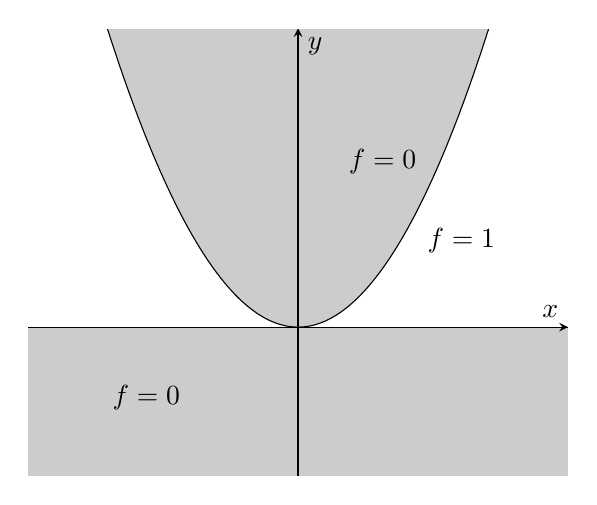
\begin{tikzpicture}
		\begin{axis}[axis x line=middle,axis y line=middle,
		xtick=\empty,ytick=\empty,
		xlabel={$x$},ylabel={$y$},
		samples=1000,
		xmin=-2,xmax=2,
		ymin=-1,ymax=2]
			\addplot[name path=P] {x^2};
			\addplot[name path=X] {0};
			\addplot[name path=B,color=white] {-1};
			\addplot[name path=C,color=white] {2};
			\addplot[fill=black, fill opacity=0.2] fill between [of=X and B];
			\addplot[fill=black, fill opacity=0.2] fill between [of=P and C];
		\end{axis}
		\node at (1.5,1) {$f=0$};
		\node at (4.5,4) {$f=0$};
		\node at (5.5,3) {$f=1$};
	\end{tikzpicture}
\end{center}
	Then we claim $f$ is continuous along all lines (line segments) through $(0,0)$ because for any direction $v=(a,b)$, $\exists \tau >0$ such that the line segment
\[
L_{v,\tau} = \{(ta,tb):|t|<\tau\}
\]
is contained in
\[
E=\{(x,y)\in \mathbb R^2 : f(x,y)=0\}=\{(x,y)\in\mathbb R^2 : y \leq 0 \text{ or } y \geq x^2\}=f^{-1}(0) .
\]
But $f$ is clearly not continuous at $(0,0)$ because
\[
\lim_{x\rightarrow 0} f\left(x,\frac12 x^2\right) = 1 \neq 0 = f(0,0) .
\]
\end{eg}

\begin{defn}[Continuity along lines, or linear continuity in some literature, but it has nothing to do with linearity of function]
	$f:\mathbb R^n \rightarrow \mathbb R^k$ is continuous along lines at $x_0 \in \mathbb R^n$ if $\forall v \in \mathbb R^n$, $t:\mathbb R \rightarrow \mathbb R^k \mapsto f(x_0+tv)$ is continuous at $t=0$, i.e.
\[
\forall v, f(x_0)=\lim_{t\rightarrow 0} f(x_0+tv).
\]
\end{defn}

\begin{eg}
	$f(x,y)=\frac{x^2y}{x^4+y^2}$ and $f(0,0)=0$ is continuous on $\mathbb R^2 \backslash \{(0,0)\}$ and along lines through $(0,0)$, but $\lim_{(x,y)\rightarrow (0,0)}$ does not exist, because
\[
\lim_{x\rightarrow 0} f(x,x^2)=\frac{x^2 x^2}{x^4+(x^2)^2} = \frac12 \neq 0 = f(0,0) .
\]
\end{eg}

The whole upshot of this is that continuity is much stronger than continuity along lines, an analogy with differentiability being much stronger than existence of directional derivative, which we are going to see later.

\section{Rudiments of topology and continuity}
\begin{defn}[Closed set]
	$X \subset \mathbb R^n$ is \textit{closed} if $x_j$ is a sequence converging to $x \in \mathbb R^n \Rightarrow x \in X$, i.e. $X$ is closed under taking limits. e.g. $\mathbb R$ is closed but $\mathbb Q$ is not.
\end{defn}
\begin{defn}[Open set]
	$U \subset \mathbb R^n$ is \textit{open} if $\forall x \in U$, $\exists \varepsilon >0$ such that $y\in \mathbb R^n$ and $|y-x|<\varepsilon \Rightarrow y\in U$, i.e. all points in $U$ have a little room to move around (can be perturbed a little) and stay in $U$.
\end{defn}

\begin{remark}[Convention]
Empty set $\varnothing$ and $\mathbb R^n$ are both open and closed.
\end{remark}

\begin{prop}
$U\subset \mathbb R^n$ is open if and only if $U^c$ is closed.
\end{prop}
\begin{proof}
Let $U \subset \mathbb R^n$ be closed and $U^c$ is nonempty. Suppose $\exists v\in U^c : \forall \varepsilon >0, |u-v|< \varepsilon \ \forall u\in U$. We can then construct a sequence $u_j\subset U$ such that $\forall \varepsilon >0, \exists N\in \mathbb N: j\geq N \Rightarrow |u_j-v|<\varepsilon ,$ i.e. $u_j\rightarrow v$. This contradicts the hypothesis that $U$ is closed. Hence $\forall v\in U^c, \exists \varepsilon >0 : |u-v|\geq \varepsilon \ \forall u\in U$, which means $\forall u\not\in U$, $|u-v|<\varepsilon$, i.e. $U^c$ is open.

Now suppose $U\subset \mathbb R^n$ is open and let $u_j \subset U^c$ be a sequence converging to $x\in \mathbb R^n$, i.e. $\forall \varepsilon >0, \exists N\in \mathbb N:j\geq N \Rightarrow |u_j-x|<\varepsilon .$ Suppose $x\in U$. But $\forall x\in U, \exists \varepsilon >0: |u-x|<\varepsilon \Rightarrow u\in U$, contradicting the hypothesis $u_j\subset U^c$. Hence $x\not\in U$, i.e. $U^c$ is closed.
\end{proof}

\begin{defn}[Open (Euclidean) ball]
Open ball of radius $r>0$, centred at $a\in \mathbb R^n$, denoted by $\mathbb B(a,r)$ or $\mathbb B_r(a)$, is $\{x\in \mathbb R^n : |x-a|<r\}$. Also $\mathbb B_r$ means $\mathbb B(0,r)$ and $\mathbb B$ is just $\mathbb B_1$, the unit ball.
\end{defn}
We can therefore rewrite Definition 3.0.2 as: $U\subset \mathbb R^n$ is \textit{open} if $\forall x\in U$, $\exists \varepsilon >0: \mathbb B(x,\varepsilon)\subset U$.

\begin{prop}
An open ball is open.
\end{prop}
\begin{proof}
Pick $y\in \mathbb B (a,r)$ and set $\delta =r-|a-y|>0$. Then we claim $\mathbb B (y,\delta ) \subset \mathbb B (a,r)$, since $x\in \mathbb B(y,\delta )$ and by triangle inequality, $|x-a|\leq |x-y|+|y-a|<\delta +|y-a| =r$.
\end{proof}

\begin{defn}[Closed ball]
$\overline{\mathbb B (a,r)}=\{x\in \mathbb R^n : |x-a|\leq r\}$.
\end{defn}
\begin{prop}
A closed ball is closed.
\end{prop}
\begin{proof}
Let $x\in \overline{\mathbb B(a,r)}^c=\{x\in \mathbb R^n:|x-a|>r\}$ and let $r_0=|x-a|-r>0.$ We claim $\mathbb B (x,r_0) \subset x\in \overline{\mathbb B(a,r)}^c$, since for any $y\in \mathbb B (x,r_0)$, $|x-a|\leq |x-y|+|y-a| \Rightarrow |y-a|\geq |x-a|-|x-y|>r .$ Therefore $\overline{\mathbb B(a,r)}^c$ is open, hence $\overline{\mathbb B(a,r)}$ is closed.
\end{proof}

\begin{prop}
Let $\{U_\lambda\}$ be a collection of open sets where $\lambda \in \Lambda $, an indexing set e.g. $\mathbb N,\mathbb Q,\mathbb R,\mathbb R^n$, etc. Then $\displaystyle \bigcup_{\lambda \in \Lambda} U_\lambda$ is open.
\end{prop}
\begin{proof}[One-liner proof! (that takes two lines to write)]
If $p\in \displaystyle \bigcup_{\lambda \in \Lambda} U_\lambda$, then $\exists \lambda^\ast : p\in U_{\lambda^\ast}$. But $U_{\lambda^\ast}$ is open, therefore $\exists \varepsilon >0 : \mathbb B(p,\varepsilon)\subset U_{\lambda^\ast} \subset \displaystyle \bigcup_{\lambda \in \Lambda} U_\lambda$.
\end{proof}

See Definition 2.1.10 and Example 2.1.11 in the typewritten notes for some fun stuff that I believe is not examinable. \\

Are intersections of open sets open? Let $U_n=\left(-\frac1n,\frac1n \right)$, then $\displaystyle \bigcap_{n\in \mathbb N} U_n=\{0\}$, which is not open. But
\begin{prop}
If the finitely many sets $U_1,\ldots,U_n$ are open then so is $\displaystyle \bigcap_{j=1}^n U_j$.
\end{prop}

\begin{proof}
Pick $p\in \displaystyle \bigcap_{j=1}^n U_j$. Then $p\in U_i \Rightarrow \exists \varepsilon_i>0 : \mathbb B (p,\varepsilon_i) \subset U_i$ for all $i\in \{1,\ldots,n\}$. Select $\varepsilon^\ast :=\min \{\varepsilon_1,\ldots,\varepsilon_n\}$ which is positive. [This is why you need it to be finite!] Then $\mathbb B (p,\varepsilon^\ast) \subset U_j$ $\forall j\in\{1,\ldots,n\}$, i.e. $\mathbb B (p,\varepsilon^\ast) \subset \displaystyle \bigcap_{j=1}^n U_j$.
\end{proof}
\begin{coro}
Arbitrary intersection of closed sets is closed; finite union of closed sets is closed.
\end{coro}
\begin{proof}
If $\{U_\lambda\}$ are closed then $\{U_\lambda^c\}$ are open and $\displaystyle \bigcup_{\lambda} U_\lambda^c$ is open, so $\displaystyle \left(\bigcup_\lambda U_\lambda^c \right)^c = \bigcap_{\lambda} U_\lambda$ is closed.

If $U_1,\ldots,U_n$ are closed then $U_1^c,\ldots,U_n^c$ are open and $\displaystyle \bigcap_{j=1}^n U_j^c$ is open, so $\displaystyle \left( \bigcap_{j=1}^n U_j^c \right)^c = \bigcup_{j=1}^n U_j$ is closed.
\end{proof}
A collection of open sets gives us what is known as a \textit{topology}.

\subsection{Continuity and topology}
Recall definition of continuity. We can translate that into ball language: $f:U\rightarrow \mathbb R^k$ is continuous at $p\in U$ if
\[
\forall \varepsilon >0, \ \exists \delta >0 : x\in \mathbb B(p,\delta ) \cap U \Rightarrow f(x)\in \mathbb B (f(p),\varepsilon ) .
\]
or equivalently
\[
f^{-1}(\mathbb B (f(p),\varepsilon))\supset \mathbb B(p,\delta) \cap U .
\]
Consider $f:\mathbb R^n \rightarrow \mathbb R^k$ (so we don't have to fuss about $\cap U$). We have
\begin{thm}[Continuity via open and closed sets]
The following statements are equivalent:\begin{enumerate}
    \item $f$ is $\varepsilon$-$\delta$ continuous at all points of $\mathbb R^n$.
    \item For all open sets $V\subset \mathbb R^k$, $f^{-1}(V)$ is open in $\mathbb R^n$.
    \item For all closed sets $\mathcal F\subset \mathbb R^k$, $f^{-1}(\mathcal F)$ is closed in $\mathbb R^n$.
\end{enumerate}
\end{thm}

\begin{proof}
\begin{itemize}
    \item[1$\Rightarrow$2:] Let $V\subset \mathbb R^k$ be open and let $p\in f^{-1}(V)$, i.e. $f(p)\in V$. Since $V$ is open, $\exists \varepsilon >0 : \mathbb B(f(p),\varepsilon) \subset V$. Continuity of $f$ at $p$ implies that $\exists \delta >0:\mathbb B(p,\delta)\subset f^{-1}(\underbrace{\mathbb B(f(p),\varepsilon)}_{\subset V})\subset f^{-1}(V)$, i.e. $f^{-1}(V)$ is open.
    \item[2$\Rightarrow$1:] Let $p\in \mathbb R^n$ and $\varepsilon >0$. Set $V:=\mathbb B(f(p),\varepsilon)$ which is open, hence $f^{-1}(V)$ is open. But $p\in f^{-1}(V)$, therefore $\exists \delta >0 : \mathbb B(p,\delta) \subset f^{-1}(V)=f^{-1} (\mathbb B (f(p),\varepsilon))$ which is exactly the $\varepsilon$-$\delta$ definition of continuity.
    \item[] 2 and 3 are obviously equivalent.
\end{itemize}
\end{proof}

Application: to show openness of a set.
\begin{eg}
\[
f(x,y)=xy\left(\sin \frac1x \right)\left(\cos \frac1y \right)
\]
is clearly continuous, therefore $\{(x,y)\in \mathbb R^2 : f(x,y)>0\}$ is open since it equals $f^{-1}((0,\infty))$ where $(0,\infty)$ is open.
\end{eg}

Now a flashback:
\subsection{Bolzano-Weierstrass theorem}
We will not go through the formal proof of B-W, which is in the typewritten notes. But an example will be demonstrated to help us understand the proof.

\begin{eg}[Review of bounded sequence in $\mathbb R$]
\[
a_j := \sin \left( \frac{\pi j}{2} \right)
\]
so we have $a_1=1,a_2=0,a_3=-1,a_4=0$ and so on. This is bounded so it has convergent subsequences, e.g. $a_{4k-3}\rightarrow 1,a_{2k}\rightarrow 0, a_{4k-1}\rightarrow -1$. Let $a_{2k}=a_{j_k}$, i.e. $j_k=2k$ which is an increasing sequence $\in \mathbb N$; this leads us to
\end{eg}
\begin{defn}[Subsequence of $a_j$]
Take $j_k$ to be an increasing sequence of natural number and then $a_{j_k}$ is a subsequence of $a_j$.
\end{defn}
\begin{eg}[Bounded sequence in $\mathbb R^2$ $(a_j,b_j)$]
\[
(a_j,b_j)=\left(\sin \frac{\pi j}{2},\sin \frac{\pi j}{3}\right)
\]
is bounded since $|(a_j,b_j)|\leq \sqrt{1^2+1^2}=\sqrt{2}$. We know $a_{2k}$ converges but $b_{2k}$ does not. But we know $b_{6l}$ converges, so we set $k_l=3l$ then $b_{j_{k_l}}=b_{j_{3l}}=b_{6l} \rightarrow 0$. Now $a_{6l}$ also converges since it's a subsequence of the convergent subsequence $a_{j_k}=a_{2k}$. So
\[
\lim_{l\infty}\left(a_{j_{k_l}},b_{j_{k_l}} \right)=(0,0).
\]
The proof (or the actual computational process) goes a bit like this: you get convergent subsequences of all the components, and take a subsequence which is a subsequence of all the convergent subsequences.
\end{eg}

\subsection{Continuity and sequential compactness}
\begin{defn}[Sequential compactness subset]
$K\subset \mathbb R^n$ is \textit{sequentially compact} if \underline{every sequence} $x_j\in K$ has a convergent subsequence $x_{j_k}$ whose limit is in $K$.
\end{defn}
\begin{defn}
$X\subset \mathbb R^n$ is bounded if $\exists M>0 : |x|\leq M \ \forall x\in X$.
\end{defn}
\begin{thm}[Heine–Borel]
$K\subset \mathbb R^n$ is sequentially compact if and only if $K$ is closed and bounded.
\end{thm}
This is a generalisation of closed bounded.
\begin{proof}
See typewritten notes.
\end{proof}
\begin{eg}[Application]
\[
S^{n-1}(a,r)=\{x\in \mathbb R^n : |x-a|=r, r>0\},
\]
the $n-1$ dimensional sphere centred at $a$ of radius $r$, is sequentially compact because it is closed: $f:\mathbb R^n \rightarrow \mathbb R, f(x)=|x-a|$ is continuous by reverse triangle inequality, then $S^{n-1}(a,r)=f^{-1}(\{r\})$ where $\{r\}$ is closed; and bounded by $|a|+r$.
\end{eg}

\begin{thm}[Continuity preserves sequential compactness]
If $f:K\rightarrow \mathbb R^k$ is continuous and $K\subset \mathbb R^n$ is sequentially compact then $f(K)$ is also sequentially compact.
\end{thm}
\begin{proof}
Straightforward. See typewritten notes.
\end{proof}

\begin{thm}[Extreme Value Theorem]
Let $K\subset \mathbb R^n$ be sequentially compact and let $f:K\rightarrow \underbrace{\mathbb R}_{\text{not }\mathbb R^k}$ be continuous. Then $\exists x_\ast, x^\ast \in K : f(x_\ast) \leq f(x) \leq f(x^\ast) \ \forall x\in K$.
\end{thm}
\begin{proof}
$f(K)$ is sequentially compact subset of $\mathbb R$. This implies $f(K)$ is closed and bounded by Theorem 3.3.3. Boundedness gives $M:=\sup f(K)$ and $m:=\inf f(K)$ are finite. By definition $\exists a_j,b_j\in f(K):\lim_{j\rightarrow \infty}a_j=M,\lim_{j\rightarrow \infty}b_j=m$. Closeness gives $M,m\in f(K)$, i.e. $\exists x^\ast, x_\ast : f(x^\ast)=M\geq f(x)\geq m=f(x_\ast).$
\end{proof}

\section{Linear maps and matrices}
Read notation on page 16 of typewritten notes.
\subsection{Norms on linear maps/matrices}
Reminder: $\mathbb R^{k\times n} \cong \mathbb R^{k n}$. Wait. So what do we gain when we write $\begin{pmatrix}a_{11} & \cdots & a_{1n} \\ \vdots & \ddots & \vdots \\ a_{k1} & \cdots & a_{kn}\end{pmatrix}$ instead of simply $(a_{11},\ldots,a_{1n},a_{21},\ldots,a_{2n},\ldots,a_{k1},\ldots,a_{kn})$? Answer is certain operations are simply form in matrix form, e.g. multiplication, taking inverses.

We then define a norm on this space as the Euclidean norm of the latter vector:
\begin{defn}[Frobenius norm]
\[
\|(a_{ij})\|_{F}:={\sqrt {\sum _{i=1}^{k}\sum _{j=1}^{n}a_{ij}^{2}}} .
\]
\end{defn}
This can also be viewed as a norm on $\mathcal L(\mathbb R^n,\mathbb R^k)$ via the identification
\[
A\in \mathcal L(\mathbb R^n,\mathbb R^k) \rightarrow \mu (A) \in \mathbb R^{k\times n},
\]
where $\mu(A)$ is the matrix representation of $A$ with respect to the standard bases on $\mathbb R^k,\mathbb R^n$. Note
\[
\mu:\mathcal L(\mathbb R^n,\mathbb R^k) \rightarrow \mathbb R^{k\times n},\quad Av_j=\sum_{i=1}^k a_{ij}w_i
\]
is a linear isomorphism.
\begin{remark}[Warning]
Sometimes we write $A$ when we mean $\mu(A)$. Context is everything.
\end{remark}
Question is given $A\in \mathbb R^{k\times n}$, how large can $|Ax|$ get relative to $|x|$ as $x$ ranges over $\mathbb R^n$? Let $x=(x_1,\ldots,x_n)$. Then
\[
|Ax|^2=\sum_{i=1}^k \left(\underbrace{\sum_{j=1}^n a_{ij}x_j}_{\text{dot product of the $i$th row with $x$}}\right)^2
\]
and by Cauchy-Schwarz
\[
|Ax|^2 \leq \sum_{i=1}^k \left(\sum_{j=1}^n a_{ij}^2\right) \left(\sum_{j=1}^n x_j^2\right)=\left(\sum_{i=1}^k \sum_{j=1}^n a_{ij}^2\right) |x|^2 = \|A\|_F^2 |x|^2.
\]
So if $x\neq 0$,
\[
\frac{|Ax|}{|x|} \leq \|A\|_F,
\]
which gives rise to
\begin{defn}[Operator norm]
\[
\|A\| := \underset{x\in \mathbb R^n\backslash\{0\}}{\sup} \frac{|Ax|}{|x|} .
\]
\end{defn}
If $x\neq 0$,
\[
\frac{|Ax|}{|x|}=\left|\frac{Ax}{|x|}\right|=\left|A\left(\frac{x}{|x|}\right)\right|,
\]
but $\left|\frac{x}{|x|}\right|=1$ since it's a unit vector. Therefore we can also write
\[
\|A\|:=\underset{x\in S^{n-1}}{\sup} |Ax|
\]
where $S^{n-1}=$ set of unit vectors $\{x\in \mathbb R^n:|x|=1\}$ which is sequentially compact. So since norm is a continuous function, it attains maximum and minimum. [See example sheet 3 for how it's useful.]

\subsubsection{Compare $\|A\|$ with $\|A\|_F$}
We have
\[
\|A\|_F^2 = \sum_{j=1}^n \sum_{i=1}^k a_{ij}^2
\]
where $a_{ij}$ is the $j$-fixed-components of $Av_j$, or $i$th column of $A$. Then
\[
\sum_{i=1}^k a_{ij}^2=|Av_j|^2 \leq \|A\||v_j|=\|A\| .
\]
So
\[
\|A\|_F^2 \leq n \|A\|^2 ,
\]
i.e.
\[
\frac{1}{\sqrt n} \|A\|_F \leq \|A\| \leq \|A\|_F .
\]
This equivalence of norms helps us deal with convergence of matrices.

\subsubsection{Properties of norm}
Read proposition 3.1.2 in typewritten notes.
\begin{prop}[Composition bound - useful]
$A\in \mathcal L(\mathbb R^n,\mathbb R^k),B\in \mathcal L(\mathbb R^k,\mathbb R^m)$. Then $BA\in \mathcal L(\mathbb R^n,\mathbb R^m)$ and $\|BA\|\leq \|B\|\|A\|$.
\end{prop}
\begin{proof}[One-liner proof!]
$|BAx|=|B(Ax)|\leq \|B\| |Ax| \leq \|B\|\|A\||x|$. So
\[
\|BA\|=\underset{x\in \mathbb R^n\backslash \{0\}}{\sup} \frac{|BAx|}{|x|} \leq \|B\|\|A\|.
\]
\end{proof}

\subsection{Convergence and continuity in $\mathcal L(\mathbb R^n,\mathbb R^k)$ / $\mathbb R^{k\times n}$}
\begin{defn}
Sequence $A_j \in \mathcal L(\mathbb R^n,\mathbb R^k)$, then
\[
\lim_{j\rightarrow \infty} A_j=A \in \mathcal L(\mathbb R^n,\mathbb R^k)
\]
if $\forall \varepsilon >0, \exists N\in \mathbb N:$
\[
j\geq N \Rightarrow \|A_j-A\|<\varepsilon \qquad \text{or, of course, }\|A_j-A\|_F<\varepsilon.
\]
\end{defn}
\begin{defn}[Ball in $\mathcal L$ (??)]
$\mathbb B(A,r)=\{B\in \mathcal L(\mathbb R^n,\mathbb R^k):\|B-A\|<r\}$.
\end{defn}

\subsubsection{Continuous matrix valued functions}
$f:\mathbb R^l\rightarrow \mathcal L(\mathbb R^n,\mathbb R^k)$ is continuous at $x\in \mathbb R^l$ if $\forall \varepsilon>0,\exists \delta>0:|y-x|<\delta \Rightarrow \underbrace{\|f(y)-f(x)\|}_{\text{Operator norm. Could use Frobenius too}}<\varepsilon .$

Okay, but what if we replace $\mathcal L(\mathbb R^n,\mathbb R^k)$ with $\mathbb R^{k\times n}\leftrightarrow \mathbb R^{nk}$? Then \begin{prop}
\[
f(x)=\begin{pmatrix}
    a_{11}(x) & \cdots & a_{1n}(x) \\
    \vdots & \ddots & \vdots \\
    a_{k1}(x) & \cdots & a_{kn}(x)
\end{pmatrix}
\]
is continuous if and only if each $a_{ij}(x)$ is continuous by equivalence of continuity and componentwise continuity.
\end{prop}

\begin{coro}
Determinant function $\Delta :\mathbb R^{n\times n}\rightarrow \mathbb R$ is continuous since each term of $\Delta (A)$ is a polynomial in the entries of $A$.
\[
\Delta(A)=a_{11}\cdots a_{nn}+\cdots
\]
in the $n^2$ variables, each of whose terms is linear in the entries $a_{ij}$ of $A$. This is an example of multilinear map.
\end{coro}

\subsection{General linear group $GL(n,\mathbb R):=\{A\in\mathcal \mathbb R^n: A\text{ is invertible}\}$}
which $=\{A\in\mathcal (\mathbb R^n): \det A\neq 0\}=\Delta ^{-1} (\mathbb R\backslash \{0\})$ where $\mathbb R\backslash \{0\} = (-\infty,0)\cup (0,\infty)$ is open, therefore $GL(n,\mathbb R)$ is an open subset of $\mathbb R^{n\times n}$. It essentially means if you jiggle an invertible matrix, it remains invertible. (Compare with singular matrices $\Delta^{-1} (0)$ which is unstable.)

\underline{Question}: given $A\in GL(n,\mathbb R)$, how large can we take $r>0$ such that $\mathbb B(A,r) \subset GL(n,\mathbb R)$?

\underline{Answer}:\begin{prop}
Let $r:=\frac{1}{\|A^{-1}\|}$. Then
\[
\mathbb B\left(A,r\right) \subset GL(n,\mathbb R).
\]
Furthermore, if $B\in \mathbb B(A,r)$, then
\[
\|B^{-1}\| \leq \frac{1}{r-\|B-A\|}.
\]
\end{prop}
\begin{proof}
Let $B\in \mathbb B(A,r)$. We know $x=A^{-1}(Ax)$. Then $|x| \leq \|A^{-1}\| |Ax|$, so $|Ax| \geq r|x|$. [Side note: This is a measure of injectivity of $A$, i.e. since $Ax=0\Rightarrow x=0$, it is a measure of how far $A$ takes a vector away from 0.] We would like to show $B$ is invertible by showing $|Bx| \geq \delta |x|$ for some $\delta>0$. We write
\[
|Bx|=|Bx-Ax+Ax| \geq |Ax|-|(B-A)x| \geq (\underbrace{r-\|B-A\|}_{\delta})|x| . \qquad (\ast)
\]
So if $B\in \mathbb B(A,r)$ $\|B-A\|<r$, then $Bx=0 \Rightarrow x=0$, i.e. $\Ker B=\{0\}$ i.e. image has same dimension $n$ by rank-nullity theorem i.e. invertible.

To estimate $\|B^{-1}\|$ we use $x=B(B^{-1})x$. By $(\ast)$, $|x|\geq (r-\|B-A\|) |B^{-1}x|$, so if $x\neq 0$, $\frac{1}{r-\|B-A\|} \geq \frac{|B^{-1}x|}{|x|}$, then take sup on right-hand side and by definition of operator norm, we have desired result.
\end{proof}

\begin{remark}
By taking $A=I_{n\times n}$, the value $r=\frac{1}{\|A^{-1}\|}$ is optimal.
\end{remark}
\begin{remark}[Linear maps are continuous]
$A\in \mathbb R^{k\times n},x\mapsto Ax: \mathbb R^n \rightarrow \mathbb R^k$ is continuous. Since $|Ax-Ay|=|A(x-y)|\leq \|A\||x-y|$. So given $\varepsilon >0$, can take $\delta = \frac{\varepsilon}{\|A\|}$ so $|x-y|<\delta \Rightarrow \|A\||x-y|<\varepsilon \Rightarrow |Ax-Ay|<\varepsilon$. So linear maps are also uniformly continuous since $\delta$ is independent of $x$.
\end{remark}
\begin{defn}[Lipschitz]
$f:U\rightarrow \mathbb R^k$ is Lipschitz if $\exists M>0$ such that $|f(x)-f(y)|<M|x-y| \ \forall x,y\in U$.
\end{defn}

\section{Derivative of $f:U\rightarrow \mathbb R^k$ where $U\subset \mathbb R^n$ is open}
Rate of change of a function of 2 or more variables depends on direction, not just the point. Simplest example: $f(x,y)=x$ changes in $x$ direction but not in $y$. We therefore introduce directional derivative, i.e. rate of change along lines. [Compare with continuity along lines.]
\subsection{Directional derivative}
Fix $x\in U$ and a direction vector $v\neq 0$ (line would be $L_{x,v}$). In principle $|v|=1$ but we'll not insist that. Parameterising $L_{x,b}$ we have $r(t):=x+tv$, and define $g_{x,v}(t):=f(x+tv)=\left. f\right|_{L_{x,v}}$. Then
\begin{defn}
\[
\partial_v f(x) = \left. \frac{\mathrm d}{\mathrm dt} g_{x,v}(t)\right|_{t=0}=\left. \frac{\mathrm d}{\mathrm dt}f(x+tv)\right|_{t=0} = \lim_{t\rightarrow 0} \frac{f(x+tv)-f(x)}{t} \in \mathbb R^k.
\]
\end{defn}
In G\&M, $\partial_v$ is denoted $D_v$.
\begin{remark}[Warning]
If $\partial_v f(x)$ exists $\forall v\in \mathbb R^n \backslash \{0\}$, then $f$ may not be continuous at $x$.
\end{remark}
\begin{eg}
Refer to Example 2.4.2. We have then $\partial_v f(0,0)=0$ since $f$ is zero for any line through $(0,0)$ but is not continuous at $(0,0)$. We need a better definition of derivative such that if it is differentiable then it is continuous!
\end{eg}

\subsection{The (Fréchet) derivative as affine linear approximation}
\begin{defn}
$\Delta :\mathbb R^n \rightarrow \mathbb R^k$ is affine linear if $\exists A\in \mathbb R^{k\times n},\ b\in \mathbb R^k : \Delta x = Ax+b$. So $b=0 \Leftrightarrow \Delta$ is linear.
\end{defn}
Recall 1-d: $f'(x) = \lim_{h\rightarrow 0} \frac{f(x+h)-f(x)}{h}$ is not possible for $h\in \mathbb R^n$ as we cannot divide by vectors. But through magic of complex numbers we can in $\mathbb R^2$. So we have two types of derivatives in $\mathbb R^2$: complex derivative, and the one we are introducing now. Of course they are related.

For which $n$'s do we have a notion for multiplication in $\mathbb R^n$? 1 and 2 of course. You may suggest cross product for 3, but bad news is $V\times V=0$. We don't want zero for nonzero vectors multiplied by themselves. But later Hamilton described quaternion $\mathbb H$, which is valid multiplication on $\mathbb R^4$, making cross product a special case. Bad news in this case is it's not commutative. Then people realised you can do multiplication in $\mathbb R^8$, i.e. Cayley numbers or octonion $\mathbb O$. ...And you stop there. Nothing more.

Back to derivative. We can rewrite the definition as
\[
\lim_{h\rightarrow 0} \frac{|f(x+h)-f(x)-hf'(x)|}{h}=0.
\]
The trick is to regard $f'(x)$ as a $1\times 1$ matrix and then $h\mapsto f'(x)h+f(x)$ is a affine linear map, which is a approximation of nonlinear map $h\mapsto f(x+h)$ fixing $x$. Then it's not hard to write the following:
\begin{defn}
$f:U\rightarrow \mathbb R^k$ is differentiable at $x\in U$ if $\exists A\in \mathcal L(\mathbb R^n,\mathbb R^k)$ such that \begin{equation}
    \lim_{h\rightarrow 0} \frac{|f(x+h)-f(x)-Ah|}{|h|}=0 .
\end{equation}
\end{defn}
This is of course equivalent to that, \begin{equation}\forall \varepsilon >0,\ \exists \delta>0 : |h|<\delta \Rightarrow |f(x+h)-f(x)-Ah| \leq \varepsilon |h|. \end{equation}

Recall for $T\in \mathcal L(\mathbb R^n,\mathbb R^k)$, $|Th| \leq \|T\| |h|$. So given nonzero $T$, we can choose $\varepsilon$ in $(2)$ so that $0<\varepsilon <\|T\|$ and $(2)$ imply that the difference between the map $h\mapsto f(x+h)$ and the affine linear map $h\mapsto Ah+f(x)$ is smaller than $|Th|$ for any linear map $T$.

We can use this to prove that linear map $A$ that satisfies the definition must be unique, if it exists at all. In other words, when $A$ satisfying definition does exist, we denote it by $D f(x)\in \mathcal L (\mathbb R^n,\mathbb R^k)$, Fréchet derivative of $f$ at $x$. We can write \begin{equation}\forall \varepsilon>0,\ \exists \delta>0 : |h|<\delta \Rightarrow |f(x+h)-f(x)-Df(x)h| \leq \varepsilon |h|.\end{equation} which essentially means that $h\mapsto Df(x)h+f(x)$ is the best affine linear approximation of $h\mapsto f(x+h)$ where $x$ is fixed.

\begin{prop}
Differentiability at $x$ implies continuity at $x$.
\end{prop}
\begin{proof}
By $(3)$ we write
\[
|f(x+h)-f(x)|\leq |f(x+h)-f(x)-Df(x)h|+|Df(x)h|\leq (\varepsilon+ \|Df(x)\|)|h| .
\]
So take
\[
\delta^\ast=\min \left\{\delta,\frac{\varepsilon}{\varepsilon+\|Df(x)\|}\right\},
\]
where $\delta$ is again from $(3)$, we then have $|h|<\delta^\ast \Rightarrow |f(x+h)-f(x)|\leq \varepsilon$.
\end{proof}

\begin{prop}[Componentwise differentiability]
$f:U\rightarrow \mathbb R^k$ is differentiable at $x$ if $f_1:U\rightarrow \mathbb R,\ldots,f_k:U\rightarrow \mathbb R$ are all differentiable at $x$ where $f(x)=(f_1(x),\ldots,f_k(x))$.
\end{prop}

\begin{prop}[Relation between derivative and directional derivative]
If $Df(x)$ exists then $\partial_v f(x)$ exists $\forall v\in \mathbb R^n$ and
\[
\partial_v f(x)=Df(x)v .
\]
In particular, if $f$ is differentiable at $x$ then $\partial_v f(x)$ is linear in $v$.
\end{prop}
\begin{proof}
Let $v\neq 0$. Set $h=tv$ in (1). So
\[
\lim_{t\rightarrow 0}\frac{|f(x+tv)-f(x)-Df(x)(tv)|}{|t||v|}=0.
\]
Multiplying by length of $|v|$ we get
\[
\lim_{t\rightarrow 0}\frac{f(x+tv)-f(x)-tDf(x)v}{t}=0.
\]
We can remove the norm since limit is zero, so limit of norm and limit of what's inside the norm is equivalent by definition. Therefore
\[
\lim_{t\rightarrow 0} \frac{f(x+tv)-f(x)}{t}=\lim_{t\rightarrow 0}\frac{tDf(x)v}{t}=Df(x)v
\]
where the left hand side is exactly the definition of $\partial_vf(x).$
\end{proof}
Linearity of $\partial_v f(x)$ means for $a,b\in \mathbb R,\ v,w\in \mathbb R^n$,
\[
\begin{aligned}\delta_{av+bw}f(x)=Df(x)(av+bw)&=aDf(x)v+bDf(x)w\\&=a\partial_v f(x)+b\partial_w f(x).\end{aligned}
\]

\subsection{Partial derivative, Jacobian matrix, gradient}
\begin{defn}
For $1\leq i\leq n$, $\partial_{v_i}f(x)$ is called $i$th \textit{partial derivative} of $f$, or $\partial_i f(x) \in \mathbb R^k$, or $f_{x_i}(x)$, where $v_i$ is the $i$th vector in standard basis.
\[
\partial_i f(x) = \begin{pmatrix}\partial_i f_1(x) \\ \vdots \\ \partial_i f_k(x)\end{pmatrix}
\]
where
\[
f(x)=\begin{pmatrix}f_1(x)\\ \vdots \\ f_k(x)\end{pmatrix}.
\]
\end{defn}
\begin{remark}
Notation like $\frac{\mathrm d f}{\mathrm d x}$ causes trouble with chain rule. Let $f(x)=\sin x$ and $g(x)=x^2$. 
\end{remark}

\begin{eg}[Compare partial derivatives with separate continuity]
Let
\[
f(x,y)=\left\{\begin{aligned}&1\qquad xy\neq 0\\&0\qquad xy=0\end{aligned} \right.
\]
(0 on axis and 1 everywhere else) Then $\partial_1 f(x,0)=0$ and $\partial_2 f(0,y)=0$. But if $v\neq (a,0),(0,b)$ then $\partial_v f(0,0)$ does not exist.
\end{eg}
\begin{defn}
$U\subset \mathbb R^n$ open, $f:U\rightarrow \mathbb R^k$. The $k\times n$ \textit{Jacobian matrix} is defined
\[
\partial f(x):=\begin{pmatrix} \partial_1 f_1(x) & \cdots & \partial_n f_1(x) \\
\vdots & & \vdots \\ \partial_1 f_k(x) & \cdots & \partial_n f_k(x) \end{pmatrix}
\]
where
\[
f(x)=\begin{pmatrix}f_1(x)\\ \vdots \\ f_k(x)\end{pmatrix}.
\]
So column-wise the matrix is
\[
\begin{pmatrix}\partial_1 f(x) & \cdots & \partial_n f(x)\end{pmatrix},
\]
list of partial derivatives of $f$, and row-wise it is
\[
\begin{pmatrix}\partial f_1(x) \\ \vdots \\ \partial f_k(x)\end{pmatrix},
\]
list of Jacobians of the components.
\end{defn}

\begin{prop}
If $Df(x)$ exists then $\partial f(x)$ exists and
\[
\underbrace{Df(x)}_{\in \mathcal L(\mathbb R^n,\mathbb R^k)}h=\underbrace{\partial f(x)}_{\in \mathbb R^{k\times n}} h .
\]
\end{prop}
\begin{remark}
$\partial f(x)$ may exist even if $Df(x)$ does not. This is why we need this proposition.
\end{remark}
\begin{proof}
For $h\in \mathbb R^n$, $h=h_1v_1+\cdots +h_n v_n$. So
\[
\begin{aligned}Df(x)h&=Df(x) \left(\sum_{i=1}^n h_i v_i\right)\\&=\sum_{i=1}^n h_i Df(x) v_i\qquad &\text{linearity} \\&= \sum_{i=1}^n h_i \partial_i f(x)\qquad &\text{Proposition 5.2.5} \\&= \partial f(x) h .\qquad &\text{column-wise definition of Jacobian}\end{aligned}
\]
\end{proof}

\subsection{Summary of different types of derivative [just a recap]}
$f:U\rightarrow \mathbb R^k,\ U\subset \mathbb R^n$ open.
\subsubsection{Directional derivative}
$\partial_h f(x),\ h\in \mathbb R^n \backslash \{0\}$ where $h$ is the `direction' (a vector in $\mathbb R^k$ not a real number) is defined
\[
\partial_h f(x) := \lim_{t\rightarrow 0}\frac{f(x+th)-f(x)}{t}=\left. \frac{\mathrm d}{\mathrm d t}(x+th) \right|_{t=0}.
\]

\underline{Geometric interpretation}: consider $g=\left.f\right|_{L_{x,h}}$, i.e. $g_{x,h}(t) := f(x+th)$, $g_{x,h}:(-\tau ,\tau) \rightarrow \mathbb R^k$ which parameterises a curve $\gamma \in \mathbb R^k$ through $f(x)=g_{x,h}(0)$. So $\partial_h f(x)=g_{x,h}' (0)=$ tangent (velocity) vector to $\gamma$ at $f(x)$

\subsubsection{Partial derivative}
It's just a special case of directional derivative.

Let $v_i$'s be the standard basis of $\mathbb R^n$, then the $i$th partial derivative $\partial_i f(x):=\partial_{v_i}f(x)$, e.g. $\partial _1 f(x) = \partial _{(1,0,\ldots,0)} f(x)$.

This is also written as $\frac{\partial f}{\partial x_i}(x)$ (because when computing, $\frac{\mathrm d}{\mathrm d t} f(x+tv_i)$ only changes the $i$th component of $x$) or $f_{x_i}(x)$.

Then we see given $h=(h_1,\ldots,h_n)$, we can write it as linear combination of standard basis $h_1v_1+\cdots+h_nv_n$, so
\[
\partial_h f(x) = \partial_{h_1v_1+\cdots+h_nv_n} f(x) \underset{\text{under condition below}}{=} h_1 \partial_1 f(x) +\cdots +h_n \partial _n f(x).
\]

If $Df(x)$ exists then $Df(x)h=\partial_h f(x)$, and so, since $Df(x)$ is linear, then
\[
\begin{aligned}\partial_h f(x) &= Df(x)h=Df(x) (h_1v_1+\cdots h_nv_n) \\&= h_1 Df(x) v_1+\cdots h_n Df(x) v_n \\&= h_1 \partial _1 f(x)+\cdots h_n \partial_n f(x).\end{aligned}
\]
In plain English, if $f$ is (Fréchet) differentiable, then $\partial _h f(x)$ is linear in $h$.

(In that case, we can know all directional derivatives just by calculating the $n$ partial derivatives.)

Reverse is clearly not true, recall the naughty function defined in Example 2.4.2.

\begin{eg}
$f:\mathbb R^2\rightarrow \mathbb R$,
\[
f(x,y)=\left\{\begin{aligned}&\frac{x^3}{x^2+y^2} \qquad &(x,y)\neq (0,0)\\ &0 \qquad &(x,y)=(0,0)\end{aligned}\right.
\]
\begin{center}
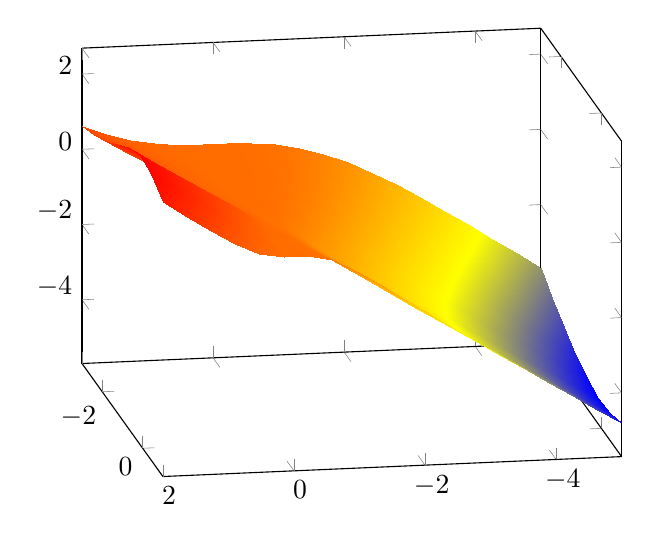
\begin{tikzpicture}
 
\begin{axis}[view = {170}{20}]
 
\addplot3 [
    domain=-5:2,
    domain y = -3:1,
    samples = 20,
    samples y = 8,
    surf,
    shader = interp] {x^3/(x^2 + y^2)};
 
\end{axis}
 
\end{tikzpicture}
\end{center}
\begin{enumerate}
    \item Calculate $\partial_v f(0,0)$.
    
    Set $v=(a,b)$. Then
\[
\partial_v f(0,0) = \lim_{t\rightarrow 0} \frac{f(ta,tb)-f(0,0)}{t}=\lim_{t\rightarrow 0} \frac{\frac{t^3a^3}{t^2a^2+t^2b^2}-0}{t}=\frac{a^3}{a^2+b^2} .
\]
    \item Calculate $\partial f(0,0)$.
    
    This is
\[
\begin{pmatrix}\partial_1 f(0,0)&\partial_2 f(0,0)\end{pmatrix}=\begin{pmatrix}\partial_{(1,0)} f(0,0)&\partial_{(0,1)} f(0,0)\end{pmatrix}=\begin{pmatrix}1&0\end{pmatrix}.
\]
    
    What you do not do is differentiate $f$ with respect to $x$ and set $x=y=0$, since it's not defined there.
    \item Calculate $\partial f(0,0)h$.
    
    This is $\begin{pmatrix}1&0\end{pmatrix} \begin{pmatrix}a\\b\end{pmatrix}=a \neq \partial _h f(0,0)$ unless $b=0$, i.e. $\partial _h f(0,0)$ not linear in $h$. Therefore $Df(0,0)$ does not exist.
    \item Calculate $f_x(x,y),\ f_y(x,y)$ where $(x,y)\neq (0,0)$.
    
    We get $f_x(x,y)=\frac{x^2(x^2+3y^2)}{(x^2+y^2)^2},\ f_y(x,y)=-\frac{2x^3y}{(x^2+y^2)^2}$. Are they continuous at $(0,0)$? We write
\[
\lim_{y\rightarrow 0} f_x (0,y) = 0\neq f_x (0,0)=1,
\]
and similarly
\[
\lim_{x\rightarrow 0} f_y (x,x) = -\frac12 \neq f_y(0,0)=0,
\]
so neither is continuous.
\end{enumerate}
\end{eg}

\subsection{Gradient of $f:U\rightarrow \mathbb R,\ U\subset \mathbb R^n$}
$f$ is real-valued not vector-valued!

We then have Jacobian matrix as a row matrix:
\[
\partial f(x) = \left(\partial _1 f(x),\ldots,\partial _n f(x)\right)
\]
which is a linear functional, i.e. a map $\mathbb R^n \rightarrow \mathbb R$. Then
\[
\partial f(x) h = \underbrace{\left(\partial _1 f(x),\ldots,\partial _n f(x)\right) \begin{pmatrix}
h_1 \\ \vdots \\ h_n
\end{pmatrix}}_{\text{matrix multiplication}} = \sum_{i=1}^n h_i \frac{\partial f}{\partial x_i} (x) .
\]
We then define the \textit{gradient} of $f$ at $x$, $\nabla f(x) = (\partial f(x))^T$, a column vector. Note that $\partial f(x) h =\underbrace{\nabla f(x) \cdot h}_{\text{dot product}}$.

\subsection{Differentiation of matrix-valued functions}
Remember $\mathbb R^{k\times n} \leftrightarrow \mathbb R^{kn}$ so there's nothing scary.
\begin{eg}
Define $f:\mathcal L(\mathbb R^n) \rightarrow \mathcal L(\mathbb R^n)$ (or $\mathbb R^{n\times n}\rightarrow \mathbb R^{n\times n}$) by $f(T)=T^2$.

We look at the special case $n=2$, so $T=\begin{pmatrix}
a & b \\ c & d
\end{pmatrix} .$ Then
\[
f(T)=T^2 = \begin{pmatrix}
a^2+bc & ab+bd \\ ca+dc & cb+d^2
\end{pmatrix} .
\]
As a map $f:\mathbb R^4 \rightarrow \mathbb R^4$, this is nothing but
\[
f(a,b,c,d) = \left(a^2+bc, ab+bd, ca+dc, cb+d^2\right).
\]
And as you can see derivative is \underline{not} $2T$. Let's use definition to differentiate $f$. Consider
\[
f(T+H)-f(T) = Df(T)H
\]
\end{eg}
and we need to guess what $Df(T)$ is. The left hand side is equal to
\[
(T+H)(T+H)-T^2 = T^2+TH+HT+H^2-T^2=TH+HT+H^2 .
\]
Just to remind you, $Df(T)$ is an element of $\mathcal L(\mathcal L(\mathbb R^n),\mathcal L(\mathbb R^n))$, so it has to be linear. We see that $TH+HT$ is linear in $H$. We then guess
\[
Df(T)H = TH+HT.
\]
We now verify the guess:
\[
\begin{aligned}
\lim_{H\rightarrow 0} \frac{\|f(T+H)-f(T)-Df(T)H\|}{\|H\|} &= \lim_{H\rightarrow 0} \frac{\|H^2\|}{\|H\|} \\ &\leq \lim_{H\rightarrow 0} \frac{\|H\|\|H\|}{\|H\|} \\ &= \lim_{H\rightarrow 0} \|H\| = 0.
\end{aligned}
\]
So we win!
Recall if $f(t)=t^2$ then $f'(t)=2t$. So we get an analogous result, different though only because matrix multiplication is not commutative.

Since we're having so much fun, why don't we calculate directional derivative $\partial_H f(T)$? We need to restrict $f'$ to the line $L_{T,H}$ through $T$ in the direction of $H$. Let $r(t):=T+tH$ and we write
\[
g_{T,H} = \left. f \right|_{L_{T,H}} = g(t) = f(r(t)) = f(T+tH) = (T+tH)^2 = T^2+t(TH+HT)+t^2H^2 .
\]
Then
\[
\partial _H f(T) = \frac{\mathrm d}{\mathrm d t} \left. f(T+tH) \right|_{t=0} = \left. TH+HT+2tH^2 \right|_{t=0} = TH+HT = Df(T)H.
\]
We just reproved that if derivative exists directional derivative is just derivative operator acting on direction, as expected.

We can also write its Jacobian matrix:
\[
\partial f (a,b,c,d)=\begin{pmatrix}
2a & c & b & 0\\
b & a+d & 0 & b\\
c & 0 & a+d & 0\\
0 & c & b & 2d
\end{pmatrix}
\]

\subsection{Chain rule}
\begin{thm}
Suppose \begin{itemize}
    \item $U \subset \mathbb R^n$ open, $V\subset \mathbb R^k$ open
    \item $f:U\rightarrow \mathbb R^k$ differentiable at $x\in U$ and $f(x)\in V$
    \item $g:V\rightarrow \mathbb R^m$ differentiable at $f(x)$
\end{itemize}
Conclusion: $g\circ f:U\rightarrow \mathbb R^m$ is differentiable at $x$ and
\[
\underbrace{(D g\circ f)}_{\in \mathcal L(\mathbb R^n, \mathbb R^m)}(x) = \underbrace{(Dg(f(x))}_{\in \mathcal L(\mathbb R^k, \mathbb R^m)} \circ \underbrace{Df(x)}_{\in \mathcal L(\mathbb R^n, \mathbb R^k)} .
\]
So we also have Jacobian form of chain rule:
\[
\begin{aligned}
\partial g\circ f(x) &= \partial g(f(x)) \cdot \partial f(x) \\ &= \begin{pmatrix}
\partial_1 g_1 (f(x)) & \cdots & \partial_k g_1 (f(x)) \\
\vdots & & \vdots \\
\partial_1 g_m (f(x)) & \cdots & \partial_k g_m (f(x)) 
\end{pmatrix}\begin{pmatrix}
\partial_1 f_1(x) & \cdots & \partial_n f_1(x) \\
\vdots & & \vdots \\
\partial_1 f_k(x) & \cdots & \partial_n f_k(x)
\end{pmatrix} .
\end{aligned}
\]
\end{thm}

\subsubsection{Common special cases}
\paragraph{Case 1: $k=m=1$.}

In this case $\partial f(x) = (\partial_1 f(x),\ldots,\partial _n f(x))$, a row vector, and $\partial g(x) = g'(x)$, a number. Then $\partial g\circ f(x) = g'(f(x)) (\partial_1 f(x),\ldots,\partial _n f(x)) .$
\begin{eg}
Calculate $\nabla (|x|)$ where $x\in \mathbb R^n \backslash \{0\}$.

Apply chain rule to $f(x) = |x|^2 = x_1^2+\cdots+x_n^2$, $g(t) = \sqrt t,\ t>0$. We write
\[
\partial f(x) = (2x_1,2x_2,\ldots,2x_n), \text{ i.e. } \nabla f(x)=2x.
\] and $g'(t) = \frac{1}{2\sqrt t}$. Then
\[
\partial |x| = \frac{1}{2\sqrt{|x|^2}} (2x_1,\ldots,2x_n) = \frac{1}{|x|} (x_1,\ldots,x_n), \text{ i.e. } \nabla |x|=\frac{x}{|x|} .
\]
\end{eg}

\paragraph{Case 2: $f:\mathbb R^n\rightarrow \mathbb R,\ r:\mathbb R\rightarrow \mathbb R^n$ (parameterisation of a curve in $\mathbb R^n$).}
We can write $r(t)=\begin{pmatrix}
x_1(t) \\ \vdots \\ x_n (t)
\end{pmatrix}$ and $f\circ r : \mathbb R \rightarrow \mathbb R$. Then
\[
\begin{aligned}
\partial f\circ r (t) &= (f\circ r)'(t) = \partial f(r(t)) r'(t) \\&= (\partial_1 f(r(t)),\ldots,\partial_n f(r(t))) \begin{pmatrix}
\frac{\mathrm d x_1}{\mathrm d t} \\ \vdots \\ \frac{\mathrm d x_n}{\mathrm d t}
\end{pmatrix} \\&= \sum_{i=1}^n \frac{\partial f}{\partial x_i} (r(t)) \frac{\mathrm d x_i}{\mathrm d t} \\&= \nabla f(r(t)) \cdot \frac{\mathrm d r}{\mathrm d t} = \nabla (f(r(t)) \cdot r'(t)
\end{aligned}
\]
\begin{eg}
Fix $x\in \mathbb R^n$ and define $r:\mathbb R\rightarrow \mathbb R^n$ by $r(t) = tx$ (a line through origin in direction of $x$).

Given $f:\mathbb R^n \rightarrow \mathbb R$, calculate $(f\circ r)'(t)$.

What is $r'(t)$? It's $x$, of course. Then
\[
(f\circ r)'(t) = \nabla f(tx) \cdot x .
\]
\end{eg}

\subsubsection{Idea of proof of chain rule (seen in first year analysis)}
We need a reformulation of definition of derivative.
\begin{lemma}
Given $f:U\rightarrow \mathbb R^k$ and $x\in U$. Since $U$ is open, $\exists r>0 : \mathbb B(x,r) \subset U.$ Also we are given a linear map $A \in \mathcal L(\mathbb R^n,\mathbb R^k)$. Then define
\[
\Delta_{x,A}f(h) = \left\{\begin{aligned}
&\frac{f(x+h)-f(x)-Ah}{|h|} \qquad &h\neq 0 \\
&0 \qquad &h=0
\end{aligned} \right.
\]
Then $f$ is differentiable at $x$ with $Df(x)=A$ if and only if $\Delta_{x,A}f$ is continuous at 0.
\end{lemma}
\begin{proof}
$\Delta_{x,A}f$ is continuous at 0 $\Leftrightarrow \lim_{h\rightarrow 0} \Delta_{x,A}f(h)=\Delta_{x,A}f(0)=0 \Leftrightarrow Df(x)$ exists and equals $A$ by definition of derivative. 
\end{proof}
\begin{notation}
If $Df(x)$ exists, abbreviate $\Delta_{x,Df(x)}f$ to $\Delta_x f$.
\end{notation}
Note that
\[
f\text{ differentiable at }x \Leftrightarrow f(x+h)=f(x)+Df(x)h+\left(\Delta_x f(x)\right)|h|
\]
and similarly
\[
g\text{ differentiable at }y \Leftrightarrow g(y+k)=g(y)+Dg(y)k+\left(\Delta_y g(y)\right)|k| .
\]
We need to show
\[
\begin{aligned}
g\circ f (x+h) &= g(f(x+h)) \\&= g(\underbrace{f(x)}_{y}+\underbrace{Df(x)h+\left(\Delta_x f(x)\right)|h|}_{k}) \\&= g(f(x))+Dg(f(x)) (Df(x)h+\Delta_x f(h) |h|) \\&\ \ \ + \left(\Delta_{f(x)}g(Df(x)h+\Delta_x f(h)|h|) \right) |Df(x)h+\Delta_x f(x)|h| |. \\&= g\circ f(x) + Dg(f(x))(Df(x)h)+\text{the rest which goes to zero}
\end{aligned}
\]
Details in the typewritten notes.

\subsection{Continuity of partial derivatives implies differentiability}
\begin{thm}
Given \begin{itemize}
    \item $f:U\rightarrow \mathbb R^k,\ U\subset \mathbb R^n$ open
    \item $x\in U$, so $\exists r>0: \mathbb B(x,r) \subset U$
    \item Jacobian matrix $\partial f(y)$ exists $\forall y\in U$
    \item $\partial f$ is continuous at $x$
\end{itemize}
then $f$ is differentiable at $x$ and
\[
Df(x)h=\partial f(x)h \quad \forall h\in \mathbb R^n .
\]
\end{thm}
\begin{remark}
$\partial f$ is continuous at $x$ if and only if $\partial_1 f_1,\ldots,\partial_n f_1,\ldots,\partial_1f_k,\ldots,\partial_n f_l$ are all continuous at $x$. So all the pathology concerning $\partial f(x)h \neq \partial_h f(x)$ can only arise if at least one of the partial derivatives is not continuous at $x$.
\end{remark}
\begin{proof}[Basic ideas in the proof] We'll demonstrate this by fixing $n=2,\ k=1$, i.e. $f(x_1,x_2) \in \mathbb R$. Full proof in appendix D in typewritten notes.

We know that if $Df(x)$ exists it satisfies
\[
\lim_{h\rightarrow 0} \frac{f(x+h)-f(x)-Df(x)h}{|h|}=0
\]
so we just need to guess what the linear map $Df(x)$ is. In particular, it follows that
\[
Df(x_1,x_2) \begin{pmatrix}
h_1 \\ h_2
\end{pmatrix} = (\partial_1f(x_1,x_2))h_1+(\partial_2f(x_1,x_2))h_2 = (\partial f(x_1,x_2)) \begin{pmatrix}
h_1 \\ h_2
\end{pmatrix} .
\]
So we consider
\[
\Delta f(h_1,h_2) := \underbrace{f(x_1+h_1,x_2+h_2)}_{f(x+h)}-\underbrace{f(x_1,x_2)}_{f(x)}-\underbrace{\left(h_1\partial_1 f(x_1,x_2)+h_2 \partial_2 f(x_1,x_2)\right)}_{\text{our guess for }Df(x)h}
\]
and we need to show
\[
\lim_{(h_1,h_2)\rightarrow (0,0)} \frac{|\Delta f(h_1,h_2)|}{|(h_1,h_2)|}=0 .
\]
If we succeed, we would manage to have two things done: prove that $f$ is differentiable, and verify that the derivative is what is has to be.

Partial derivatives provide information only along lines parallel to axes. So we go from $(x_1,x_2)$ to $(x_1+h_1,x_2+h_2)$ via $(x_1+h_1,x_2)$.

\begin{center}
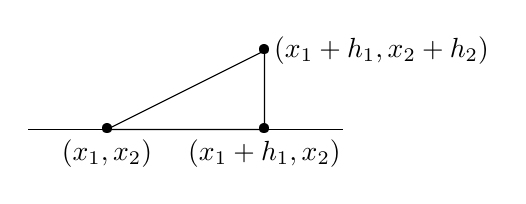
\begin{tikzpicture}[scale=2]
 \draw (0.5,0) -- (2.5,0);
 \draw (1,0)node{\textbullet}node[anchor=north]{$(x_1,x_2)$} -- (2,0)node{\textbullet}node[anchor=north]{$(x_1+h_1,x_2)$} -- (2,0.5)node{\textbullet}node[anchor=west]{$(x_1+h_1,x_2+h_2)$} -- (1,0);
\end{tikzpicture}
\end{center}

Computationally this means
\[
\begin{aligned}
&\quad \ f(x_1+h_1,x_2+h_2)-f(x_1,x_2) \\&= \underbrace{f(x_1+h_1,x_2+h_2)-f(x_1+h_1,x_2)}_{\text{II}}+\underbrace{f(x_1+h_1,x_2)-f(x_1,x_2)}_{\text{I}} \\
&= h_2\partial_2 f(x_1+h_1,x_2+\theta_2h_2) + h_1\partial_1 f(x_1+\theta_1h_1,x_2) \qquad \text{for some } \theta_1,\theta_2\in (0,1) \text{ by MVT}
\end{aligned}
\]
So
\[
\begin{aligned}
\Delta f(h_1,h_2)=&h_1 \left[\partial_1 f(x_1+\theta_1h_1,x_2)-\partial_1 f(x_1,x_2) \right]\\&+h_2 \left[\partial_2 f(x_1+h_1,x_2+\theta_2h_2)-\partial_2 f(x_1,x_2) \right]
\end{aligned}
\]
and by continuity of $\partial f(x_1,x_2)$, given $\varepsilon >0,$
\[
\exists \delta>0: 0<|(\tilde{h_1},\tilde{h_2})|<\delta \Rightarrow |\partial f(x_1+\tilde{h_1},x_2+\tilde{h_2})-\partial f(x_1,x_2)|<\varepsilon.
\]
And we know that if $|(h_1,h_2)|<\delta$ then we also have 
\[
|(x_1+\theta_1h_1,x_2)| = \theta_1 |h_1| \leq \theta_1 |(h_1,h_2)| <\theta_1\delta<\delta
\]
and
\[
|(x_1 + h_1 , x_2 + \theta_2h_2) - (x_1 , x_2)| = \sqrt{(h_1)^2 + (\theta_2h_2)^2} \leq |(h_1,h_2)| < \delta.
\]
so we have
\[
|\partial_1 f(x_1+\theta_1h_1,x_2)-\partial_1 f(x_1,x_2)|\leq |\partial f(x_1+\theta_1h_1,x_2)-\partial f(x_1,x_2)| <\varepsilon
\]
and similarly
\[
|\partial_2 f(x_1+h_1,x_2+\theta_2h_2)-\partial_2 f(x_1,x_2)| <\varepsilon .
\]
So as long as $0<|(h_1,h_2)|<\delta$ we have
\[
\frac{|\Delta f(h_1,h_2)|}{|(h_1,h_2)|} \leq \frac{\varepsilon(|h_1|+|h_2|)}{\sqrt{h_1^1+h_2^2}} < 2\varepsilon .
\]
\end{proof}

\begin{prop}[Very useful]
$f:U\rightarrow \mathbb R^k$ is continuously differentiable at all points of $U$, i.e.
\[
x\mapsto Df(x):U\rightarrow \mathcal L(\mathbb R^n,\mathbb R^k) \text{ is continuous } \forall x\in U
\]if and only if
\[
x\mapsto \partial f(x):U\rightarrow \mathbb R^{k\times n} \text{ is continuous } \forall x\in U.
\]
\end{prop}

\begin{remark}
Recall that by equivalence of norms, a function $F:U\rightarrow \mathcal L(\mathbb R^n,\mathbb R^k)$ is continuous (with respect to operator norm) if and only if $\mu(F):U\rightarrow \mathbb R^{k\times n}$ is continuous (with respect to Frobenius norm).
\end{remark}
\begin{proof}
Suppose $Df(x)$ is continuous at all points $x\in U$. Then $\partial f(x) = \mu (Df(x))$ is continuous at all points $x\in U$. This follows immediately from the remark.

Now suppose $\partial f(x)$ is continuous at all points $x\in U$. This is slightly trickier because we don't know if $Df(x)$ exists or not, so we cannot directly apply the remark. But fortunately by Theorem 5.8.1, it does. So $Df(x)$ is continuous at all points $x\in U$ by continuity of $\partial f$.
\end{proof}
We can now check existence and continuity of $Df$ simply by checking those of $\partial f$, which is just A-level stuff.
\begin{notation}
$C^1(U,\mathbb R^k) = \{f:U\rightarrow \mathbb R^k \ |\  \partial f:U\rightarrow \mathbb R^k\text{ is continuous}\}$.

$C^1(U,\mathbb R)$ is abbreviated to $C^1(U)$.
\end{notation}

\subsection{Mean value inequality (MVI)}
Recall 1-d MVT: $\exists c\in (x,y): \frac{f(y)-f(x)}{y-x}=f'(c).$ It's more useful in this form: if $|f'(u)|\leq M \ \forall u\in (x,y)$ then $\underbrace{|f(y)-f(x)| \leq M|y-x|}_{MVI}$, i.e. Lipschitz.
\begin{prop}[Generalised MVI]
Given $x,y \in U$ open, suppose $\exists$ a continuously differentiable path $r:[a,b] \rightarrow U$ such that $r(a)=x,\ r(b)=y$. Suppose $f\in C^1 (U,\mathbb R^k)$ and that $\exists M\geq 0$ such that $\|\partial f(u)\|\leq M \ \forall u\in U$. Then $|f(x)-f(y)|\leq M \ \text{length} (C_{xy})$ where $C_{xy}=r([a,b])$.
\end{prop}
\begin{proof}
We have
\[
f(y)-f(x) = f(r(b))-f(r(a)) \overbrace{=}^{\text{FTC}} \int_a^b \frac{\mathrm d}{\mathrm d t} f(r(t)) \ \mathrm d t
\]
where $\int_a^b g(t) \ \mathrm d t := \left( \int_a^b g_1(t) \ \mathrm d t,\ldots, \int_a^b g_k(t) \ \mathrm d t \right).$ How do we differentiate that? Chain rule of course:
\[
=\int_a^b \partial f(r(t)) \cdot r'(t) \ \mathrm d t
\]
So
\[
\begin{aligned}
|f(y)-f(x)| &\leq \int_a^b \left| \partial f(r(t)) \cdot r'(t) \right| \ \mathrm d t \leq \int_a^b \|\partial f(r(t)) \| |r'(t)| \ \mathrm d t \\ &\leq M \int_a^b |r'(t)| \mathrm d t \qquad \text{by assumption} \\& = M \ \text{length} (C_{xy}) \qquad \text{by definition of length}
\end{aligned}
\]
\end{proof}
\begin{defn}[Path connectedness]
$U\subset \mathbb R^n$ is \textit{(differentiably) path connected} if $\forall p,q \in U,\ \exists$ a continuously differentiable path $r:[a,b]\rightarrow U$ such that $r(a)=p,\ r(b)=q$.
\end{defn}
It's really a notion in topology. Differentibility doesn't make much sense in those things since it implies some kind of linear structure. This is why differentiably is with parentheses. We'll see a lot more about this in Norms, Metrics and Topologies.

\begin{coro}[Vanishing derivative]
Suppose $U\subset \mathbb R^n$ is differentiably path connected and $f:U\rightarrow \mathbb R^k$ satisfies $\partial f(x)=0 \ \forall x\in U$. Then $f$ is constant on $U$.
\end{coro}
\begin{proof}
Fix $y\in U$. Given another $x\in U, \ \exists r:[a,b]\rightarrow U:r(a)=x,\ r(b)=y$. Then $f(y)-f(x) =\int_a^b \underbrace{\partial f(r(t))}_{0} r'(t) \ \mathrm d t = 0$, i.e. $f(x)=f(y) \ \forall x\in U$.
\end{proof}

\begin{defn}
$U\subset \mathbb R^n$ is \textit{convex} if $\forall x,y\in U$, the straight line $L_{xy}$ joining $x$ to $y$ is contained in $U$.
\end{defn}
\begin{coro}[Mean value inequality]
$U\subset \mathbb R^n$ is convex. If $f\in C^1(U,\mathbb R^k)$ and $\|\partial f(x)\| \leq M \ \forall x\in U$. Then $|f(x)-f(y)|\leq M|x-y|$.
\end{coro}
\begin{remark}
$f$ being Lipschitz does not imply that $\|\partial f(x)\| \leq M$, nor does it imply $f$ is differentiable. e.g. $f(x)=|x|$ or $\frac{x^3}{x^2+y^2}$.
\end{remark}

\section{Vector fields, curves, line integrals}
This is mainly review from MA134.
\begin{defn}
A \textit{vector field} $\underline{v}$ on $U\in \mathbb R^n$ is a function $\underline{v}:U\rightarrow \mathbb R^n$, $\underline{v}(x)=\left(v_1(x_1,\ldots,x_n),\ldots,v_n(x_1,\ldots,x_n)\right)$.
\end{defn}
Why is $\underline{v}$ underlined? To view $\underline{v}(x)$ as ``attached'' at $x$.
\begin{eg}
Consider $\underline{v}(x,y)=(x,y).$ You would view this as a map, in fact the identity map. But we want to view it as a whole bunch of vectors attached to every vector in $\mathbb R^2$.
\begin{center}
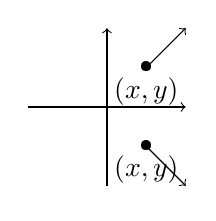
\begin{tikzpicture}
\draw[->] (-1,0) -- (1,0);
\draw[->] (0,-1) -- (0,1);
\draw[->] (0.5,0.5)node[anchor=north]{$(x,y)$} node{\textbullet} -- (1,1);
\draw[->] (0.5,-0.5)node[anchor=north]{$(x,y)$} node{\textbullet} -- (1,-1);
\end{tikzpicture}
\end{center}

Also consider $\underline{v}(x,y) = \frac{1}{x^2+y^2} (x,y)$, so the length of the vector attached to $(x,y)$ is $\frac{1}{\sqrt{x^2+y^2}}$, i.e. it decays.
\end{eg}

\subsection{Components of a vector}
Let $e\in \mathbb R^n$ be a unit vector. Given $v\in \mathbb R^n$ set $v^{\tan}= (v\cdot e) e$. Observe
\[
(v-v^{\tan})\cdot e - v\cdot e - (v\cdot e)(e\cdot e)=0,
\]
i.e. $v-v^{\tan} \perp e$. So we set $v^\perp :=v-v^{\tan}$ and $v=v^{\tan} + v^\perp$.

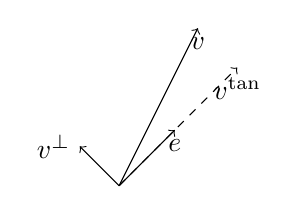
\begin{tikzpicture}
\draw[->] (0,0) -- (1,2)node[anchor=north]{$v$};
\draw[->] (0,0) -- (0.7071,0.7071)node[anchor=north]{$e$};
\draw[->,dashed] (0,0) -- (1.5,1.5)node[anchor=north]{$v^{\tan}$};
\draw[->] (0,0) -- (-0.5,0.5)node[anchor=east]{$v^\perp$};
\end{tikzpicture}

\subsection{Curves and their parameterisation}
\begin{defn}
A \textit{curve} $C$ is a \underline{subset of $\mathbb R^n$} which can be realised as the image of a continuous map $r:\underset{\text{could also be }[0,\infty)\text{ etc.}}{[a,b]}\rightarrow \mathbb R^n$, which is called \underline{a} (not unique!) \textit{parameterisation} of $C$.
\end{defn}

\begin{eg}
$C=$line through $0\in \mathbb R^2 \perp (a,b) = \{(x,y):ax+by=0\}$. A natural parameterisation of $C$ would be $r(u)=(-bu,au)$. But we can also take something like $r(u) = -b \sinh u + a\sinh u$.
\end{eg}
Parameterisation is a kinematic description of how a point $u\in [a,b]$ moves along $C$. Definition of curve allows weird examples like space-filling curves. We want to restrict ourselves to non-weird curves:
\begin{defn}
A \textit{regular} curve is one which admit \textit{regular} parameterisation:
\begin{itemize}
    \item $r$ is continuously differentiable
    \item $r'(u)\neq 0 \ \forall u\in [a,b]$ \qquad (you cannot momentarily stop)
\end{itemize}
\end{defn}

Read appendix F of typewritten notes for demystification of arc length.

Consider regular $C$ with parameterisation $r:[a,b]\rightarrow \mathbb R^n$. Length of segment of $C$ between $r(a)$ and $r(u)$ is denoted $s(u)$,
\[
s(u) := \int_a^u |r'(\tau)| \ \mathrm d \tau .
\]
But how do we know it does not depend on different parameterisation? By change of variables formula:
\[
\frac{\mathrm d s}{\mathrm d u} \underbrace{=}_{\text{FTC}} |r'(u)|\underbrace{>0}_{\text{regular}},\qquad s(a)=0
\]
this is an initial value ODE problem which has a solution (but typically cannot be solved explicitly).

Let $L=$ length of $C=s(b)$. Then $s:[a,b]\rightarrow [0,L]$ is clearly bijection by monotonicity. So the inverse exists, and we call it $u$ (since the function is a point in the domain interval). Note that $u(s(u))=u,\ s(u(s))=s.$ We then can give the following definition:
\begin{defn}
\textit{Arc length parameterisation} $\rho$ of $C$ is defined by
\[
\rho (s) = r(u(s)).
\]
\end{defn}
Note by chain rule
\[
\frac{\mathrm d \rho}{\mathrm d s} = r'(u(s)) \frac{\mathrm d u}{\mathrm d s} = \frac{\overbrace{r'(u(s))}^{\text{view as function of }u}}{\frac{\mathrm d s}{\mathrm d u}},
\]
i.e. $\rho'(s(u))=\frac{r'(u)}{|r'(u)|}$, a unit vector, i.e. arc length parameterisation is unit speed, i.e. $\rho'(s)=t(s)=$unit tangent to $C$ at $\rho(s)$.
\subsection{Line integral}
\begin{defn}
Given $f\in C(\mathbb R^n)$ and regular curve $C\subset \mathbb R^n$, the \textit{line integral} of $f$ along $C$ is defined
\[
\int_C f \ \mathrm d s := \int_0^L f(\rho(s)) \ \mathrm d s.
\]
\end{defn}
But we've been warned that this is in general not computable. So what do we do? Note
\[
\int_0^L f(\rho(s)) \ \mathrm d s \underbrace{=}_{\text{change variable to }u} \int_a^b f(r(u)) \frac{\mathrm d s}{\mathrm d u} \mathrm d u = \int_a^b f(r(u)) |r'(u)| \ \mathrm d u,
\]
which is the computation formula of line integral, and does not depend on choice of $r$ as long as its regular.

\begin{defn}
Given continuous vector field $\underline v(s)$ and a regular curve $C\subset \mathbb R^n$. The \textit{tangential line integral} of $\underline v$ along $C$ is defined
\[
\int_C (\underline v\cdot t)\ \mathrm d s.
\]
\end{defn}
\begin{remark}
$\underline v\cdot t>0$ means $v$ points along $t$ and $\underline v\cdot t<0$ means $\underline v$ points against $t$. Now $\displaystyle \frac{\int_C \underline v \cdot t \ \mathrm d s}{\int_C 1 \ \mathrm d s}$ is the average of $\underline v\cdot t$ along $C$ where the denominator is just length of $C$. So
\[
\int_C \underline v \cdot t \ \mathrm d s= (\text{length of } C) \underbrace{(\text{average of }\underline v\cdot t \text{ along }C)}_{\text{how much ``on avergae'' }\underline v\text{ points along }C}
\]
To compute this we change variables again:
\[
=\int_a^b \underline v(r(u)) \cdot \frac{\mathrm d r}{\mathrm d u} \mathrm d u.
\]
\end{remark}
\begin{defn}
If $C$ is a closed curve in $\mathbb R^n$ then
\[
\ointctrclockwise_C \underline v \cdot \mathrm d r
\]
is often called the \textit{circulation} of $\underline v$ around $C$ (because this is positive if, on average, $\underline v$ flows around $C$). The arrow indicates curve is oriented.
\end{defn}

Circulation around rectangle $R=[\alpha,\beta]\times [\xi,\eta] \subset \mathbb R^2$

\begin{center}
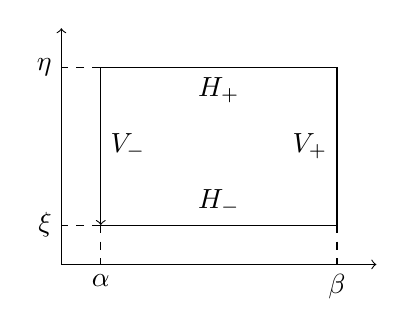
\begin{tikzpicture}
\draw[->] (0,0) -- (4,0);
\draw[->] (0,0) -- (0,3);
\draw[->] (0.5,0.5) --node[auto]{$H_{-}$} (3.5,0.5) --node[auto]{$V_{+}$} (3.5,2.5) --node[auto]{$H_{+}$} (0.5,2.5) --node[auto]{$V_-$} (0.5,0.5);
\draw[dashed] (0.5,0.5) -- (0.5,0)node[anchor=north]{$\alpha$};
\draw[dashed] (0.5,0.5) -- (0,0.5)node[anchor=east]{$\xi$};
\draw[dashed] (3.5,0.5) -- (3.5,0)node[anchor=north]{$\beta$};
\draw[dashed] (0.5,2.5) -- (0,2.5)node[anchor=east]{$\eta$};
\end{tikzpicture}
\end{center}

If we parameterise $H_{-}$ we have $r(x) = (x,\xi),\ \alpha \leq x\leq \beta$ and
\[
\int_{H_-} \underline v \cdot \mathrm d r = \int_\alpha^\beta \underline v (r(x)) \cdot r'(x) \ \mathrm d x = \int_\alpha^\beta (a(x,\xi),b(x,\xi)) \cdot (1,0) \ \mathrm d x = \int_\alpha^\beta a(x,\xi) \ \mathrm d x .
\]
And similarly for $V_+$ we have $r(y)=(\beta,y)$ and
\[
\int_{V_+} \underline v \cdot \mathrm d r = \int_\xi^\eta b(\beta, y) \ \mathrm d y ,\qquad \int_{H_+} \underline v \cdot \mathrm d r = -\int_\alpha^\beta a(x,\eta) \ \mathrm d x
\]
and so for $V_-$
\[
\int_{V_-} \underline v \cdot \mathrm d r = -\int_\xi^\eta b(\alpha ,y) \ \mathrm d y
\]
and finally
\[
\begin{aligned}
\ointctrclockwise _R \underline v \cdot \mathrm d r &= \int_\alpha^\beta (a(x,\xi)-a(x,\eta)) \ \mathrm d x + \int_\xi^\eta (b(\beta,y)-b(\alpha,y)) \ \mathrm d y \\ &= \int_\alpha^\beta \left( -\int_\xi^\eta \frac{\partial a}{\partial y} (x,y) \ \mathrm d y \right) \mathrm d x+\int_\xi^\eta \left( \int_\alpha^\beta \frac{\partial b}{\partial x} (x,y) \ \mathrm d x \right) \mathrm d y \qquad \text{by FTC} \\
&= \iint_R \left( \frac{\partial b}{\partial x}-\frac{\partial a}{\partial y} \right) \underbrace{\mathrm dA_{x,y}}_{\text{in Euclidean it's just }\mathrm d x \mathrm d y}. \qquad \text{by Fubini}
\end{aligned}
\]
This is Green's theorem in its most specific case. We want to extend this to general regions. First question is what direction should we go? Orientation of boundary is tricky. We formulate these questions with some definitions first.
\begin{defn}
A bounded open subset $\Omega \subset \mathbb R^n$ is called a \textit{region} if $\exists f:\mathbb R^n \rightarrow \mathbb R$ such that
\begin{enumerate}
    \item all partial derivatives of $f$ exist and are continuous
    \item $\Omega = \{x\in \mathbb R^n : f(x) <0\} = f^{-1} ((-\infty,0))$
    \item $\nabla f(p) \neq 0 \ \forall p\in f^{-1}\{0\}$
\end{enumerate}
$f$ is called a \textit{defining function} of $\Omega$.
\end{defn}
Condition 3 implies for $p\in f^{-1}\{0\}$ we can set $n_+ (p) = \frac{\nabla f(p)}{|\nabla f(p)|}$ which is perpendicular to $f^{-1}\{0\}$ by proof we've seen in MA134. Then $\exists \delta >0: f(p+tn_+ (p)) >0 \ \forall t\in (0,\delta)$ and $f(p+tn_+ (p)) <0 \ \forall t\in (-\delta,0)$. (To see this see Q5 of Ex 6). Geometrically, $n_+ (p)$ is outward unit normal and $f^{-1}\{0\}$ is \textit{boundary} of $\Omega$, denoted $\partial \Omega$.

\begin{eg}
$f(x,y,z) = x^2+y^2+z^2-4$. Then $\Omega = f^{-1} ((-\infty,0)) = \{x^2+y^2+z^2 <4\}=$ ball centred at $(0,0)$ of radius 2, and $\partial \Omega = \{0\}=S^2(2).$ Also $\nabla f = (2x,2y,2z) \neq (0,0,0)$ when $(x,y,z) \in \partial \Omega$, and $n_+ (x,y,z) = \frac1{2\sqrt{x^2+y^2+z^2}} (2x,2y,2z) = \frac12 (x,y,z)$.
\end{eg}

If we are in $\mathbb R^2$, $f^{-1}\{0\}$ would be a regular curve and in $\mathbb R^3$ it's a regular surface. This requires implicit function theorem which will be proved near the end of term. Now we focus in $\mathbb R^2$.

\begin{defn}
Given region $\Omega \in \mathbb R^2$, $p\in \Omega$ and $n_+ (p) = (h(p),k(p)).$ Rotate $n_+$ by $\frac{\pi}{2}$ anticlockwise to get \textit{positively oriented tangent} $t_+(p):=(-k(p),h(p))$.
\end{defn}

\begin{thm}[Green's theorem in plane]
Denote $\Omega \cup \partial \Omega$ as $\overline{\Omega}$ (called \textit{closure} of $\Omega$), which is a subset of $U\subset \mathbb R^2$ open. Given vector field $\underline v \in C^1 (U,\mathbb R^2),\ \underline v(x,y) = \left(a(x,y),b(x,y)\right)$, define
\[
\curl \underline v (x,y) := \frac{\partial b}{\partial x}-\frac{\partial a}{\partial y}.
\]
Then
\[
\iint_\Omega \curl \underline v \ \mathrm d A = \ointctrclockwise_{\partial \Omega} \underline v \cdot t_+ \ \mathrm d s \underbrace{=}_{\text{computationally}} \ointctrclockwise \underline v \cdot \mathrm d r,
\]
where $s$ is an arc length parameterisation of $\partial \Omega$ and $s$ is a positively oriented parameterisation of $\partial \Omega$, i.e. $\frac{r'}{|r'|} = t_+$.
\end{thm}

Wait... the specific rectangle case is not a region by definition. So we extend the $\Omega$ in Green's theorem to \textit{piecewise region}. (Similarly in analysis, if a function is only finitely different than a uniformly continuous function it's still integrable.)
\begin{proof}[Strategy of proof]
Approximate $\Omega$ by a rectangle mesh $R_\varepsilon$ such that area of $(\Omega \backslash R_\varepsilon) < \varepsilon$, then
\[
\iint_{R_\varepsilon}\curl \underline v \ \mathrm d A \rightarrow \iint_\Omega \curl \underline v \ \mathrm d A
\]
since their difference is at most $\underset{\Omega}{\max} \{\curl \underline v\} \varepsilon$, which can be attained since $\curl$ is continuous. After this we need to see Green's theorem holds for $R_\varepsilon$ due to cancellation:
\begin{center}
\begin{tikzpicture}
\draw[->] (0,0) -- (1,0);
\draw (1,0) -- (1,0.7) -- (0,0.7) -- (0,0);
\draw (0.5,-1) -- (1.5,-1) -- (1.5,0);
\draw[->] (1.5,0) -- (0.5,0);
\draw (0.5,0) -- (0.5,-1);
\end{tikzpicture}
\end{center}
Finally we need to show
\[
\int_{\partial R_\varepsilon} \underline v \cdot t \ \mathrm d s \rightarrow \int_{\partial \Omega} \underline v \cdot t \ \mathrm d s,
\tag{$\ast$}
\]
which is not at all obvious! We all know why the proof of $\pi= 4$ is invalid, right? We cannot simply approximate curves by stairs, i.e. sum of length of stairs is not $C^1$ convergence. So we need to proceed with more caution.

Parameterise $\partial \Omega$ by $r:[\alpha,\beta]\rightarrow \mathbb R^2$, partition $[\alpha,\beta]$ into
\[
[\underset{=u_0}{\alpha},u_1],[u_1,u_2],\ldots,[u_{l-1},\underset{=u_l}{\beta}].
\]
and set $\gamma_j = r\left( \left[ u_{j-1},u_j\right]\right),\ 1\leq j\leq l.$ Then
\[
\begin{aligned}
\int_{\partial \Omega} \underline v \cdot \mathrm d r &= \sum_{j=1}^l \int_{\gamma_j} \underline v \cdot \mathrm d r \approx \sum_{j=1}^l \underline v (r(u_j)) \cdot (r(u_{j+1})-r(u_j)) \\
&=\sum_{j=1}^l \left(a(r(u_j)),b(r(u_j)) \right) \cdot \left( \Delta x_j,\Delta y_j \right) \\
&=\sum_{j=1}^l \left(a(r(u_j)),b(r(u_j)) \right) \cdot \left( \Delta x_j,0 \right)+\sum_{j=1}^l \left(a(r(u_j)),b(r(u_j)) \right) \cdot \left(0,\Delta y_j \right) \\
&\approx \int_{\Gamma_j} \underline v \cdot \mathrm d r
\end{aligned}
\]
where $\Gamma_j$ denotes the relevant part of boundary of $R_\varepsilon$.

\begin{center}
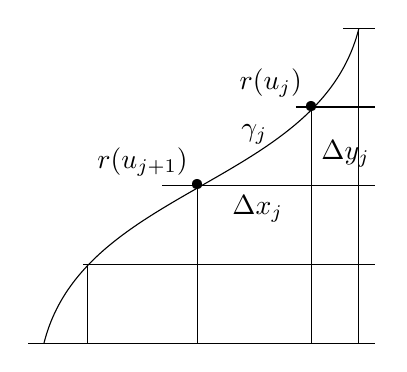
\begin{tikzpicture}
\draw (0,0) .. controls (0.5,2) and (3.5,2) .. (4,4)node[pos=0.63,anchor=south] {$\gamma_j$};

\draw (-0.2,0) -- (4.2,0);
\draw (0.5,1) -- (4.2,1);
\draw (1.5,2) -- (4.2,2)node[pos=0.45,anchor=north]{$\Delta x_j$};
\draw (3.2,3) -- (4.2,3);
\draw (3.8,4) -- (4.2,4);

\draw (0.55,1) -- (0.55,0);
\draw (1.95,2)node{\textbullet} node[anchor=south east]{$r(u_{j+1})$} -- (1.95,0);
\draw (3.4,3)node{\textbullet} node[anchor=south east]{$r(u_j)$} -- (3.4,0) node[pos=0.2,anchor=west]{$\Delta y_j$};
\draw (4,4) -- (4,0);
\end{tikzpicture}
\end{center}
Now we can show that $\varepsilon \rightarrow 0$ we have $(\ast).$

The modern argument uses something cleverer called partition of unity which again reduces Green's theorem to a rectangle, done in manifolds. (Breaking up functions to simpler ones is easier than breaking up domains.)
\end{proof} 

\subsection{Flux and divergence in $\mathbb R^2$}
If $v=(a,b),$ define $v^\perp := (b,-a)=$ clockwise rotation of $v$ by $\frac{\pi}{2}$, we have
\begin{itemize}
    \item $v\cdot w = v^\perp \cdot w^\perp$
    \item $\left(v^\perp\right)^\perp = -v$
    \item if $n_+$ is outward unit normal then $t_+ = -n_+^\perp$
\end{itemize}
So clearly this $\perp$ has some nice properties. Natural question is what's Green's theorem applied to $v^\perp$? If $\underline v (x,y) = (a(x,y),b(x,y))$ then
\[
\curl \underline v^\perp =\curl (b,-a) = \frac{\partial}{\partial x} (-a) - \frac{\partial}{\partial y} b = -\left( \frac{\partial a}{\partial x}+\frac{\partial b}{\partial y}\right).
\]
This leads to
\begin{defn}
The \textit{divergence} of $\underline v$, denoted $\nabla \cdot \underline v$ or $\text{div } \underline v$, is
\[
\frac{\partial a}{\partial x}+\frac{\partial b}{\partial y} \qquad \text{or written as} \qquad \left( \frac{\partial}{\partial x},\frac{\partial}{\partial y} \right) \cdot (a,b).
\]
\end{defn}
So
\begin{thm}[Divergence (Gauss's) theorem (and its proof)]
\[
\begin{aligned}
\iint_\Omega \nabla \cdot \underline v \ \mathrm d A &= -\iint_\Omega \curl \underline v^\perp \ \mathrm d A \\&= -\ointctrclockwise_{\partial \Omega} \underline v^\perp \cdot t_+ \ \mathrm d s \qquad \text{by Green's} \\&=-\ointctrclockwise_{\partial \Omega} \underline v^\perp \cdot (-n_+^\perp) \ \mathrm d s \\&= \underbrace{\ointctrclockwise_{\partial \Omega} \underline v\cdot n_+ \ \mathrm d s}_{\text{flux}} .
\end{aligned}
\]
\end{thm}

\begin{eg}
We have 2 vector fields $\underline w(x,y) = (x,y)$ and $\underline v (x,y) = \frac{1}{x^2+y^2} (x,y).$ Then
\[
\begin{aligned}
\nabla \cdot \underline w &= \frac{\partial}{\partial x} x+\frac{\partial}{\partial y}y = 2 \\
\nabla \cdot \underline v &=\frac{\partial}{\partial x} \frac{x}{x^2+y^2}+\frac{\partial}{\partial y}\frac{y}{x^2+y^2} = 0.
\end{aligned}
\tag{$\ast$}
\]
Now let $C_1$ be unit circle. We want to calculate flux of $\underline v$ across $C_1$. Clearly $n_+(x,y)=(x,y)$, so on $C_1$,
\[
\underline v(x,y)\cdot n_+(x,y) = \frac{1}{x^2+y^2}(x,y)\cdot (x,y)=1.
\]
Therefore the flux is
\[
\int_{C_1} 1 \ \mathrm d s = \text{length of }C_1 = 2\pi.
\]
This is not a contradiction of the above theorem. It's tempting to say by $(\ast)$, $\displaystyle \iint_{\text{disk}} \nabla \cdot \underline v \ \mathrm d A$ is 0, but in fact this integral doesn't exist at all since the field is not bounded.

What's the flux across $C_2$ the circle of radius 2? Clearly $n_+(x,y) = \frac12 (x,y),$ so the flux is
\[
\int_{C_2} \underline v \cdot n_+ \ \mathrm d s = \int_{C_2} \frac14 (x,y) \cdot \frac12 (x,y) \ \mathrm d s = \int_{C_2} \frac12 \ \mathrm d s = \text{half of length of }C_2 = 2\pi.
\]
Let's apply divergence theorem to the annulus $\Omega = \{(x,y) : 1\leq x^2+y^2\leq 2\}$ where $\underline v$ is continuously differentiable to see why the two fluxes we calculated are the same:
\[
\begin{aligned}
\iint_{\Omega} \nabla \cdot \underline v \ \mathrm d A &= \int_{\partial \Omega} \underline v \cdot n_+ \ \mathrm d s \\&= \int_{C_2} \underline v \cdot n_+ \ \mathrm d s + \int_{C_1} \underline v \cdot \overbrace{n_+}^{\text{opposite to the previous one}} \ \mathrm d s \\&= 0.
\end{aligned}
\]
\begin{center}
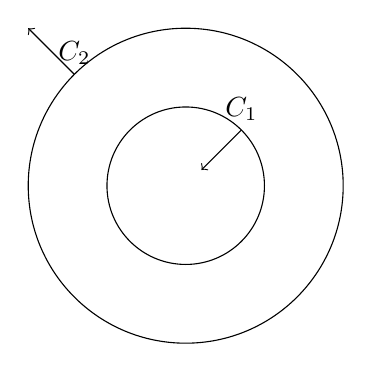
\begin{tikzpicture}
\draw (0,0) circle (1cm);
\draw (0,0) circle (2cm);
\draw[->] (0.707,0.7071)node[anchor=south]{$C_1$} -- (0.2,0.2);
\draw[->] (-1.414,1.414)node[anchor=south]{$C_2$} -- (-2,2);
\end{tikzpicture}
\end{center}
\end{eg}

\subsection{Flux and divergence in $\mathbb R^3$}
We need notion of element of area $\mathbb d A$ of a parameterised regular surface (we want a tangent plane, or more simply its normal vector everywhere).

\begin{defn}
Consider $r:\mathcal O\rightarrow \mathbb R^3$ where $\mathcal O$ is an open subset. $r(u,v) = (x(u,v),y(u,v),z(u,v))$ is a \textit{regular} parameterisation of surface $S=r(\mathcal O)$ if
$r$ is continuously differentiable and \[
\frac{\partial r}{\partial u} \times \frac{\partial r}{\partial v} (u,v) \neq 0 \qquad \forall (u,v) \in \mathcal O .
\]
i.e. $\displaystyle \frac{\partial r}{\partial u}, \frac{\partial r}{\partial v}$ are linearly independent and tangent plane $T_{r(u,v)}S$ of $S$ at $r(u,v)$ is spanned by $\displaystyle \frac{\partial r}{\partial u}, \frac{\partial r}{\partial v}$.
\end{defn}
\begin{defn}
\textit{Element of area} $\mathrm d A_{u,v}$ on $S$ is
\[
\left| \frac{\partial r}{\partial u} \times \frac{\partial r}{\partial v} (u,v) \right|  \mathrm d u \ \mathrm d v ,
\]
which is independent of parameterisation by change of variables.
\end{defn}
The intuition behind this the area can be written as
\[
\Delta S(u,v) = r(\Delta R_{u,v})
\]
where area of $\Delta R_{u,v}$ is just $\Delta u \times \Delta v.$ Then area of $\Delta S(u,v)$ is approximately
\[
\left| \frac{\partial r}{\partial u}\Delta u \times \frac{\partial r}{\partial v}\Delta v\right|=\left| \frac{\partial r}{\partial u} \times \frac{\partial r}{\partial v}\right|\Delta u\ \Delta v .
\]
We can't simply use polyhedral to approximate surfaces similar to what we've done for lines: see Schwarz lantern.

Now given continuous $f:\mathbb R^3 \rightarrow \mathbb R$, we can define surface integral
\[
\iint_S f \ \mathrm d A := \iint_{\mathcal O} f(r(u,v)) \left| \frac{\partial r}{\partial u} \times \frac{\partial r}{\partial v} (u,v) \right|  \mathrm d u \ \mathrm d v .
\]
And we can do flux.
\begin{defn}
Given vector field $\underline v (x,y,z)$ across surface $S$, \textit{flux} is defined by
\[
\iint_S \underline v \cdot n \ \mathrm d A = \iint_{\mathcal O} \underline v (r(u,v)) \cdot \frac{\partial r}{\partial u} \times \frac{\partial r}{\partial v}  \mathrm d u \ \mathrm d v
\]
where $n$ is normal to $S$. The left hand side notation emphasises independence of parameterisation, and since we can write
\[
n=\frac{\frac{\partial r}{\partial u} \times \frac{\partial r}{\partial v}}{\left|\frac{\partial r}{\partial u} \times \frac{\partial r}{\partial v}\right|},\qquad \mathrm d A = \left|\frac{\partial r}{\partial u} \times \frac{\partial r}{\partial v}\right| \mathrm d u \ \mathrm d v,
\]
cancellation of these leads to the right hand side computational formula and proves independence of parameterisation.
\end{defn}
How to interpret this? Think of $\underline v$ as velocity with which piece of surface $\Delta S_{u,v}$ moves. We look at how a small area, approximated by a parallelogram $\Delta \sigma (u,v)$, moves in time to $\Delta \tilde{\sigma}(u,v).$ It sweeps out a volume enclosed by the two surfaces and the ``walls'' parallel to $\underline v \Delta t$. So amount of volume that flows across $S$ in time $\Delta t$ is just
\[
\left(\iint_{S} \underline v \cdot n \ \text{Area}(\Delta \sigma (u,v)) \right)\Delta t
\]
and rate is
\[
\iint_{S} \underline v \cdot n \ \text{Area}(\Delta \sigma (u,v)) = \iint_S \underline v \cdot n \ \mathrm d A.
\]

\begin{thm}[Divergence theorem for regions in $\mathbb R^3$]
Given solid region $\Omega \subset \mathbb R^3$ and open subset $U\subset \mathbb R^3$ such that $\overline{\Omega}=\Omega \cup \partial \Omega \subset U$, and $\underline v:U\rightarrow \mathbb R^3$ is $C^1$ vector field, then
\[
\iiint_\Omega \nabla \cdot \underline v \ \mathrm d V = \iint_{\partial \Omega} \underline v \cdot n_+ \ \mathrm d A = \iint_{\mathcal O} \underline v (r(u,v)) \frac{\partial r}{\partial u} \times \frac{\partial r}{\partial v} \ \mathrm d u \ \mathrm d v.
\]
where $\nabla \cdot v$ is similarly defined to Definition 6.4.1, $n_+$ is outward unit normal to $\Omega$ and $r$ is a positively oriented parameterisation of $\partial \Omega$ in sense that $\frac{\frac{\partial r}{\partial u} \times \frac{\partial r}{\partial v}}{\left|\frac{\partial r}{\partial u} \times \frac{\partial r}{\partial v}\right|} = n_+$.
\end{thm}

See example in notes and example sheets.

\subsection{Gradient fields}
\begin{defn}
$\underline v : U \rightarrow \mathbb R^n$ is a \textit{gradient field} if $\exists f \in C^1 (U) :$
\[
\underline v (x) = \nabla f (x) \quad \forall x\in U,
\]
so in components
\[
v_1(x) = \frac{\partial f}{\partial x_1}(x),\ldots,v_n(x) = \frac{\partial f}{\partial x_n}(x),
\]
where $\underline v (x) = \left(v_1 (x),\ldots,v_n(x) \right)$.
\end{defn}
\begin{thm}[FTC for gradient fields]
Given $f\in C^1(U)$, curve $C_{pq}\subset U$ parameterised by a continuously differentiable $r:[a,b]\rightarrow U : r(a)=p,\ r(b)=q$. Then
\[
\int_{C_{pq}} \nabla f \cdot \mathrm d r = f(q)-f(p) .
\]
\end{thm}
\begin{remark}
The usual FTC is
\[
\int_p^q f'(t) \ \mathrm d t = f(q)-f(p).
\]
\end{remark}
\begin{proof}
\[
\begin{aligned}
\int_{C_{pq}} \nabla f \cdot \mathrm d r &= \int_a^b \nabla f (r(u)) \cdot \frac{\mathrm d r}{\mathrm d u} \ \mathrm d u \\ &= \int_a^b \frac{\mathrm d }{\mathrm d u} f(r(u)) \ \mathrm d u \qquad \text{chain rule} \\&= f(r(a))-f(r(b)) \qquad \text{FTC} \\&= f(q)-f(p).
\end{aligned}
\]
\end{proof}
\begin{coro}[Independence of path; stronger than that of parameterisation]
Given 2 arbitrary different paths $C_{pq}$ and $\tilde{C}_{pq}$ between $p,q$, we have
\[
\int_{C_{pq}} \nabla f \cdot \mathrm d r=\int_{\tilde{C}_{pq}} \nabla f \cdot \mathrm d r .
\]
\end{coro}
\begin{coro}
\[
\oint_C \nabla f \cdot \mathrm d r = 0
\]
for all closed curves $C\subset U$ (does not have to be embedded).
\end{coro}
Take any point on the curve as both $p$ and $q$ and we can see this.
\subsection{Conservative fields}
\begin{defn}
$\underline v:U\rightarrow \mathbb R^n$ is \textit{conservative} if
\[
\oint_C \nabla f \cdot \mathrm d r = 0
\]
for all closed curves $C\subset U$.
\end{defn}
So all gradient fields are conservative. What about the converse?
\begin{prop}
$\underline v$ is conservative if and only if $\int_{C_{pq}} \underline v \cdot \mathrm d r$ is independent of choice of path in $U$ from $p$ to $q$.
\end{prop}
\begin{proof}
\begin{itemize}
    \item[$\Rightarrow:$] We need to show
    \[
    \int_{C_{pq}} \nabla f \cdot \mathrm d r=\int_{\tilde{C}_{pq}} \nabla f \cdot \mathrm d r
    \]
    for two arbitrary paths. Denote $\tilde{C}_{pq}$ with opposite orientation as $-\tilde{C}_{pq}$. Then $C_{pq} \cup -\tilde{C}_{pq} = C$ is closed (go from $p$ to $q$ along $C_{pq}$ and from $q$ back to $p$ along opposite direction of $\tilde{C}_{pq}$). So
    \[
    \oint_C \nabla f \cdot \mathrm d r = \int_{C_{pq}} \underline v \cdot \mathrm d r + \int_{-\tilde{C}_{pq}} \underline v \cdot \mathrm d r = 0.
    \]
    Hence
    \[
    \int_{C_{pq}} \underline v \cdot \mathrm d r=-\int_{-\tilde{C}_{pq}} \underline v \cdot \mathrm d r=\int_{\tilde{C}_{pq}} \underline v \cdot \mathrm d r
    \]
    \item[$\Leftarrow:$] Let $C$ be a closed curve and $p\in C$. What are the paths from $p$ to $p$? Along the closed curve, and just don't go anywhere and stay at $p$.
    \[
    \begin{aligned}
    \oint_C \underline v \cdot \mathrm d r &= \int_{C_{pp}}\underline v \cdot \mathrm d r \\&=\int_{C_p^\ast} \underline v \cdot \mathrm d r \qquad \text{by independence of path} \\&= \int_0^1 \underline v (r(u)) \cdot \underbrace{\frac{\mathrm d r}{\mathrm d u}}_{=0}  \mathrm d u \\&=0 ,
    \end{aligned}
    \]
    where $C_p^\ast$ is the constant path: $r(u) = p \ \forall u\in [0,1]$.
\end{itemize}
\end{proof}
\subsection{Scalar potential of conservative fields}
Given $\underline v (x) = (v_1(x),\ldots,v_n(x)),\ x=(x_1,\ldots,x_n)$, is there $f:U\rightarrow \mathbb R:\nabla f(x) = \underline v(x)$? i.e. Can we solve the following $n$-partial differential equations?
\[
\frac{\partial f}{\partial x_1}(x)=v_1(x),\ldots,\frac{\partial f}{\partial x_n}(x)=v_n(x) .
\]
We have $n$ equations for 1 unknown function. Too many equations! If $n=1$, we just have $\frac{\mathrm d f}{\mathrm d x} = v(x)$ so $f(x) \int^x v(u) \ \mathrm d u$.
\begin{thm}
A continuous vector field $\underline v:U\rightarrow \mathbb R^n$ is a gradient field if and only if $\underline v$ is conservative.
\end{thm}
\begin{remark}
You would say this is not very helpful. Checking if a vector field is conservative is painful: you need to check infinite number of closed curves.
\end{remark}
\begin{proof}[Sketch of proof]
Gradients fields are conservative by definition of latter. So we suppose $\underline v$ to be conservative and find a way to construct $f$ in Definition 6.6.1. The $n=1$ case gives us a hint: we do this by integration, in particular line integral along arbitrary paths from $p$ to $q$ in $U$.

Fix $q\in U$. Assume $U$ is path connected. So given $p\in U$, $\exists$ a (non unique) path $C_{qp}\subset U$. Then define
\[
f(p):=\int_{C_{qp}} \underline v \cdot \mathrm d r.
\]
$\underline v$ being conservative ensures that $f$ is well-defined, in the sense that it does not depend on choice of $C$. Now we need to check $\nabla f(x) = \underline v (x)$, i.e. $\displaystyle \frac{\partial f}{\partial x_i} (x) = v_i(x)$ for all $i=1,\ldots,n$. Since
\[
\begin{aligned}
f(x+he_i) &=\int_{C_{qx}} \underline v \cdot \mathrm d r + \int_{L_i} \underline v \cdot \mathrm d r  \\&= f(x) + \int_0^h \underline v (x+te_i) \cdot e_i \ \mathrm d t \\&= f(x) + \int_0^h v_i (x+t e_i) \ \mathrm d t ,
\end{aligned}
\]
we have
\[
\frac{\partial f}{\partial x_i} (x) = \lim_{h\rightarrow 0} \frac{f(x+he_i)-f(x)}{h} = \lim_{h\rightarrow 0} \frac{\int_0^h v_i (x+te_i) \ \mathrm d t}{h} = v_i(x)
\]
\begin{center}
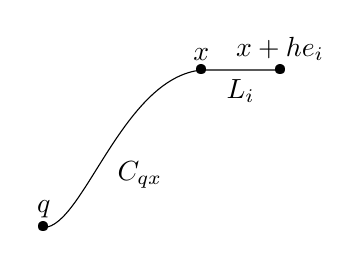
\begin{tikzpicture}
\draw (0,0)node[anchor=south]{$q$}node{\textbullet} .. controls (0.5,0.01) and (1,1.9) .. (2,2)node[anchor=south]{$x$}node{\textbullet} node[pos=0.5,anchor=north west]{$C_{qx}$} -- (3,2)node[anchor=south]{$x+he_i$}node{\textbullet} node[pos=0.5,anchor=north]{$L_i$};;
\end{tikzpicture}
\end{center}
\end{proof}
\begin{eg}[Explicit calculation of scalar potential of a conservative vector field on $\mathbb R^n$]
$\underline v (x,y,z) = \left(xye^{xy}+e^{xy}+1,x^2 e^{xy},2z\right)$. We want to find $f:\underline v = (f_x,f_y,f_z)$, i.e. solve 3 equations. Starting with the easiest one,
\[
\frac{\partial f}{\partial z} = 2z \Rightarrow f(x,y,z)=z^2\underbrace{+h(x,y)}_{\text{the ``constant''}},
\]
then
\[
\frac{\partial}{\partial y} \left(z^2+h(x,y) \right) = \frac{\partial h}{\partial y} = x^2 e^{xy} \Rightarrow h(x,y) = xe^{xy}+g(x),
\]
finally
\[
\begin{aligned}
\frac{\partial}{\partial x} \left(z^2+xe^{xy}+g(x) \right) &= e^{xy}+xye^{xy} + \frac{\partial g}{\partial x} = xye^{xy}+e^{xy}+1 \\ &\Rightarrow g=x+C.
\end{aligned}
\]
We conclude that
\[
f(x,y,z) = z^2+xe^{xy}+x+C.
\]
This process exploits the niceness of $\mathbb R^n$. We can of course use the recipe constructed in the proof above to find $f$, but would run into nasty integrals.
\end{eg}
\begin{eg}[What goes wrong if $\underline v$ is not conservative?]
$\underline v(x,y)=(0,x)$. We need
\[
\frac{\partial f}{\partial x} = 0 \Rightarrow f(x,y)=g(y)
\]
and
\[
\frac{\partial f}{\partial y} = \frac{\mathrm d g}{\mathrm d y} =x
\]
which is impossible.
\end{eg}
\subsubsection{Relation of curl and existence of scalar potential for $C^1$ vector fields}
Suppose $f\in C^2(\Omega),\ \Omega \in \mathbb R^2$. Then $\frac{\partial^2 f}{\partial x \partial y}=\frac{\partial^2 f}{\partial y \partial x}$ and this can be written as
\[
\frac{\partial}{\partial x} \left( \frac{\partial f}{\partial y} \right) - \frac{\partial}{\partial y} \left( \frac{\partial f}{\partial x} \right) =0,
\]
i.e. $\curl \nabla f = 0$. (So if $\curl \underline v \neq 0$ then $\underline v$ is not conservative, a useful indicator.) Converse is true, only locally, i.e. if $\underline v \in C^1(U)$ and $\curl \underline v= 0$ on $U$, then
\[
\forall x\in U,\ \exists p>0: \mathbb B(x,p) \subset U \text{ and } \exists f \in C^2 (\mathbb B(x,p)) : \nabla f(y)=\underline v (y) \ \forall y \in \mathbb B(x,p).
\]
However, there may not exist a global scalar potential $f\in C^2(U)$ such that $\underline v(y) = \nabla f(y) \ \forall y\in U$ (see Q2 in assignment 4) unless the first homology group $H_1(\Omega,\mathbb R)=\{0\}$ is trivial. This is something that measures 1-d holes. $\Omega$ being simply connected, i.e. $\pi_1(\Omega)=1$, is sufficient for this.
\subsection{Incompressible and conservative vector fields}
Consider fluid with density $\rho (x,t)$ and velocity $v(x,t)$ at position $x$ at time $t$. They satisfy the continuity equation
\[
\frac{\partial \rho}{\partial t}+\nabla \cdot (\rho \underline v)=0,
\]
which can be viewed as infinitesimal conservation of mass. Assume fluid is in compressible (e.g. water at low pressure and constant temperature). Then $\rho$ is constant and by above equation $v$ satisfies $\nabla \cdot v=0$.
\begin{defn}
Using synecdoche we call such $v$ \textit{incompressible} fields, also \textit{solenoidal} fields in context of electromagnetism (also \textit{divergence-free} in context of, well, mathematics).
\end{defn}
Suppose $\underline v$ conservative, i.e. $\underline v =\nabla f$. Then if $\nabla \cdot \underline v=0$ then $\nabla \cdot (\nabla f)=0$, i.e.
\[
\left( \frac{\partial}{x_1},\ldots,\frac{\partial}{\partial x_n} \right) \cdot \left( \frac{\partial f}{\partial x_1},\ldots,\frac{\partial f}{\partial x_n} \right) =0,
\]
so
\[
\frac{\partial ^2 f}{\partial x_1^2}+\cdots +\frac{\partial ^2 f}{\partial x_n^2} =: \Delta f = 0
\]
\begin{defn}
$\Delta$ is called the Laplace operator or \textit{Laplacian}, and such $f$ are called \textit{harmonic}.
\end{defn}

\begin{eg}[of harmonic functions]
\begin{itemize}
    \item linear functions $f(x) = a\cdot x$ where $a=(a_1,\ldots,a_n) \in \mathbb R^n$. We have $\nabla f(x)=a$.
    \item real/imaginary parts of $\mathbb C$-analytic functions, e.g. $f(z)=z^2=x^2-y^2+2ixy$. Then $x^2-y^2$ and $2xy$ are both harmonic: consequence of Cauchy–Riemann
\end{itemize}
\end{eg}
We seek radial harmonic functions on $\mathbb R^2\backslash \{0\}$.
\begin{defn}
$f:\mathbb R^n \backslash \{0\} \rightarrow \mathbb R$ is \textit{radial}/\textit{spherically symmetric} if $\exists \varphi:\mathbb R_{>0} \rightarrow \mathbb R: f(x) = \varphi (|x|)$. (i.e. $f$ is constant on circles)
\end{defn}
If $f$ is radial, then
\[
\nabla f(x) = \varphi'(|x|) \nabla (|x|) = \varphi' (|x|) \underbrace{\frac{x}{|x|}}_{\text{unit radial vector}}
\]
\begin{prop}[Zero flux property of divergence-free vector fields] 
If $\underline v \in C^1 (U,\mathbb R^3)$ is divergence-free, then the flux
\[
\iint_{\partial \Omega} \underline v \cdot n_+ \ \mathrm d A=0
\]
for all region $\Omega:\overline{\Omega}\subset U$.
\end{prop}
\begin{proof}
Immediately from divergence theorem.
\end{proof}
Now notice that $f$ harmonic is the same as $\nabla f$ divergence-free. So we can apply zero flux property with
\[
\Omega = A_R = \mathbb B_R \backslash \overline{\mathbb B}_1 = \left\{ x\in \mathbb R^2 : 1 <|x| <R \right\}
\]
and
\[
\partial A_R = C_R \cup C_1
\]
\begin{center}
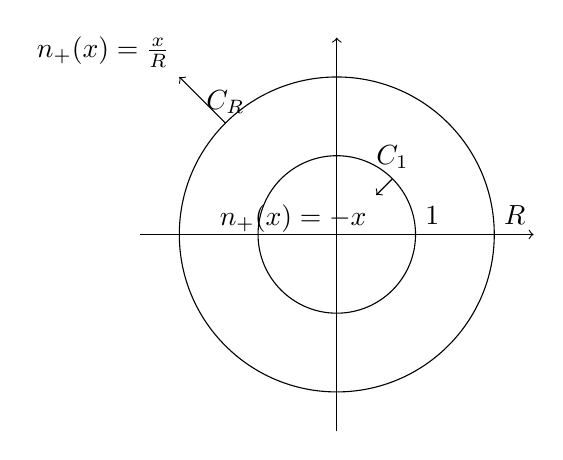
\begin{tikzpicture}
\draw (0,0) circle (1cm);
\draw (0,0) circle (2cm);
\draw[->] (-2.5,0) -- (2.5,0);
\draw[->] (0,-2.5) -- (0,2.5);
\node[anchor=south west] at (1,0) {1};
\node[anchor=south west] at (2,0) {$R$};
\draw[->] (0.707,0.7071)node[anchor=south]{$C_1$} -- (0.5,0.5)node[anchor=north east]{$n_+(x)=-x$};
\draw[->] (-1.414,1.414)node[anchor=south]{$C_R$} -- (-2,2)node[anchor=south east]{$n_+ (x) = \frac{x}{R}$};
\end{tikzpicture}
\end{center}
by writing
\[
\begin{aligned}
0&=\int_{\partial A_R} \nabla f \cdot n \ \mathrm d s = \int_{C_R} \varphi'(R) \frac{x}{R} \cdot \frac{x}{R} \ \mathrm d s + \int_{C_1} \varphi'(1) x \cdot (-x) \ \mathrm d s \\
&=\varphi'(R) \int_{C_R} \mathrm d s - \varphi'(1) \int_{C_1} \mathrm d s \\
&= \varphi'(R) 2\pi R-\varphi'(1) 2\pi
\end{aligned}
\]
So $\varphi$ satisfies the ODE
\[
\varphi'(R) = \frac{\varphi'(1)}{R}
\]
i.e. $\varphi(R) = \varphi'(1) \log R+C$. So $f(x) = a\log (|x|)+b$.

\section{Inverse function theorem}
\subsection{1-d review}
Assume
\begin{itemize}
    \item $f:(a,b) \rightarrow \mathbb R$ is differentiable on $(a,b)$ and $f'(x)>0 \ \forall x\in (a,b)$
\end{itemize}
Then
\begin{enumerate}
    \item $f$ is increasing (MVT)
    \item $f:(a,b)\rightarrow (\alpha,\beta)$ is a bijection where $\displaystyle \alpha:=\lim_{x\downarrow a+}f(x)$ and $\displaystyle \beta:=\lim_{x\uparrow b-}f(x)$ exist because of $(i)$. Surjection from IVT
    \item $f^{-1}:(\alpha,\beta)\rightarrow (a,b)$ is differentiable and
    \[
    \left(f^{-1}\right)' (y) = \frac{1}{f'\left(f^{-1}(y)\right)} .
    \]
\end{enumerate}
Alternative formulation of 2. and 3.: set $y=f(x)$ and view this as an equation for $x$ in terms of $y$, then
\begin{enumerate}
    \item[2.] $y=f(x)$ can be solved for $x$ in terms of $y$, i.e. $x=f^{-1}(y)$
    \item[3.] \[
    \frac{\mathrm d x}{\mathrm d y} (y) = \frac{1}{\frac{\mathrm d y}{\mathrm d x} \left(f^{-1}(y)\right)}
    \]
\end{enumerate}
\begin{eg}
$f(x)=e^x=y$. Solve for $x$ and we have $x=\log y = f^{-1}(y)$, and
\[
\frac{\mathrm d x}{\mathrm d y} = \frac{1}{y} = \frac{1}{e^{\log y}} = \frac{1}{\frac{\mathrm d y}{\mathrm d x} (\log y)}.
\]
\end{eg}

We want to extend these results to higher dimensions. We start with linear cases which are the simplest. A linear map $T:\mathbb R^n \rightarrow \mathbb R^n$ is a bijection if and only if $\det T\neq 0$. Then we can solve $Tx=y$ for $x:x=T^{-1}y$. Also $DT=T$ since... well if approximate a linear function linearly you get the function itself. This \underline{suggests} that a continuously differentiable map $\psi:\mathbb R^n \rightarrow \mathbb R^n$ \underline{may} be a bijection if $\det \partial \psi (x) \neq 0 \ \forall x\in \mathbb R^n$. Some evidence this may be true:

Recall assignment 2 Q2. We were given \begin{itemize}
    \item $f\in C^1 (\mathbb B,\mathbb R^k)$ where $\mathbb B$ is the unit ball in $\mathbb R^n$
    \item $Df(0)$ is injective, i.e. (Example sheet 3 Q5) $\exists \alpha>0: |Df(0)h| \geq \alpha |h| \ \forall h\in \mathbb R^n$.
\end{itemize}
We conclude $\exists \delta>0: f$ is injective on $\mathbb B_{\delta}$. Quantitatively $|f(x)-f(y)| \geq \frac{\alpha}{2} |x-y| \ \forall x,y\in \mathbb B_\delta$.

\begin{eg}
We view the complex function $f(z) =e^z$ as $\psi:\mathbb R^2 \rightarrow \mathbb R^2$ defined by $\psi (x,y) = \left( e^x \cos y , e^x \sin y \right)$. Then its Jacobian is
\[
\partial \psi (x,y) = \begin{pmatrix}
    e^x \cos y & -e^x \sin y \\ e^x \sin y & e^x \cos y
\end{pmatrix}
\]
and $\det \partial \psi (x,y) = e^{2x}>0 \ \forall (x,y)\in \mathbb R^2$. But $\psi$ is not injective; in fact, it's periodic.
\end{eg}
Seems that we arrive at the wrong conclusion. The insight that the above question recalled gives us is that maybe we don't have a global inverse from $\det \partial \neq 0$ yet: we just have a \textit{local inverse}.
\begin{defn}
A \textit{neighbourhood} $\mathcal N_p$ of $p$ is any open set that contains $p$.
\end{defn}
\begin{defn}
$\psi:U\rightarrow V$ is a \textit{local bijection} at $p\in U$ if $p$ has a neighbourhood $\mathcal N_p \subset U$ and $q:=\psi (p)$ has a neighbourhood $\mathcal N_q \subset V : \psi : \mathcal N_p \rightarrow \mathcal N_q$ is a bijection.
\end{defn}
\begin{thm}[Inverse function]
Given \begin{itemize}
    \item $\psi \in C^1 (U,\mathbb R^n),\ U\subset \mathbb R^n$ open
    \item $D\psi (p)$ invertible at $p\in U$, i.e. $\det \partial \psi(p)\neq 0$
\end{itemize}
and set $q=\psi(p)$, we have \begin{itemize}
    \item $\exists$ a neighbourhood $\mathcal N_p$ and $\mathcal N_q : p\in \mathcal N_p, \ q\in \mathcal N_q \subset \psi(U)$ and $\psi:\mathcal N_p \rightarrow \mathcal N_q$ is a bijection
    \item $\psi^{-1}:\mathcal N_q \rightarrow \mathcal N_p$ is continuously differentiable and
    \[
    D\psi^{-1}(y) = \left(D\psi \left(\psi^{-1}(y)\right)\right)^{-1} \quad \forall y \in \mathcal N_q .
    \tag{$\ast$}
    \]
\end{itemize}
Informally this means $\psi(x)=y$ can be solved for $x$ and $x=\psi^{-1}(y) \ \forall y \in \mathcal N_q$.
\end{thm}
\begin{proof}[Proof of $\ast$]
We already have $\psi^{-1}$ exists and is continuously differentiable. So differentiate both sides of
\[
\psi \left( \psi^{-1} (y) \right)=y \quad \forall y \in \mathcal N_q
\]
to get
\[
\underbrace{D\psi \left(\psi^{-1}(y)\right) \cdot D\psi^{-1}(y)}_{\text{chain rule}} = I_n
\]
which gives what's desired immediately.
\end{proof}
\begin{eg}
$\psi(x,y)=\left(e^x+e^y,y\right) = \left(u(x,y),v(x,y)\right)$. To compute $\psi^{-1}$, we solve $e^x+e^y=u,\ y=v$ for $x,y$ in terms of $u,v$: $y(u,v)=v$ and $x(u,v)=\log \left(u-e^v\right)$, so
\[
\psi^{-1}(u,v) = \left(\log \left(u-e^v\right),v\right) = (x(u,v),y(u,v)).
\]
This is case where the inverse is explicitly calculable. What the inverse function theorem tells us that even if that's not the case, nevertheless a solution exists.
\end{eg}
\begin{eg}
$U=\{(x,y):|x|,|y| < \frac{\pi}{2}\}$, and $\psi:U\rightarrow \mathbb R^2$ is defined by $\psi(x,y)=(xy,\cos x+ \cos y)$.

Inverse function theorem tells us to calculate Jacobian first, so:
\[
\partial \psi (x,y) = \begin{pmatrix}
    y & x \\ -\sin x & -\sin y
\end{pmatrix}
\]
and
\[
\det \partial \psi (x,y) = x\sin x-y\sin y=0 \text{ when }x=y\text{ or }x=-y.
\]
In fact $\psi (x,y) = \psi (-x,-y) = \psi (y,x) = \psi(-y,-x)$. Take $p_1=\left(0,\frac{\pi}{3}\right)$, and if we set symmetries $p_2=\left(\frac{\pi}{3},0\right),\ p_3=\left(0,-\frac{\pi}{3}\right),\ p_4=\left(-\frac{\pi}{3},0\right)$ then $\psi(p_1)=\psi(p_2)=\psi(p_3)=\psi(p_4)$, so $\psi$ is clearly not injective.
\begin{center}
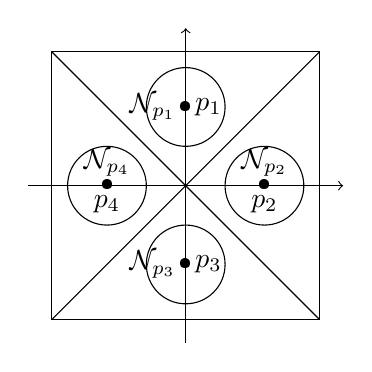
\begin{tikzpicture}
\draw[->] (-2,0) -- (2,0);
\draw[->] (0,-2) -- (0,2);
\draw (-1.7,-1.7) -- (-1.7,1.7) -- (1.7,1.7) -- (1.7,-1.7) -- (-1.7,-1.7);
\draw (-1.7,-1.7) -- (1.7,1.7);
\draw (-1.7,1.7) -- (1.7,-1.7);
\draw (0,1)node{\textbullet} node[anchor=west]{$p_1$} circle (0.5)node[anchor=east]{$\mathcal N_{p_1}$};
\draw (1,0)node{\textbullet} node[anchor=north]{$p_2$} circle (0.5)node[anchor=south]{$\mathcal N_{p_2}$};
\draw (0,-1)node{\textbullet} node[anchor=west]{$p_3$} circle (0.5)node[anchor=east]{$\mathcal N_{p_3}$};
\draw (-1,0)node{\textbullet} node[anchor=north]{$p_4$} circle (0.5)node[anchor=south]{$\mathcal N_{p_4}$};
\end{tikzpicture}
\end{center}
But what inverse function theorem tells us that there are local neighbourhoods $\mathcal N_{p_i}$ where bijections exist. What we get is 4 branches of inverses of the same function on 4 different domains (like positive and negative square roots as 2 inverses of $x\mapsto x^2$). We can't explicitly write them but we know their derivatives:
\[
\partial \psi_1 ^{-1} \left(0,\frac32\right) = \left( \partial \psi \left(0,\frac{\pi}{3}\right) \right)^{-1} = \begin{pmatrix}
    \frac{\pi}{3} & 0 \\ 0 & -\frac{\sqrt3}{2}
\end{pmatrix}^{-1} = \begin{pmatrix}
    \frac{3}{\pi} & 0 \\ 0 & -\frac{2}{\sqrt3}
\end{pmatrix}
\]
and
\[
\partial \psi_2 ^{-1} \left(0,\frac32\right) = \left( \partial \psi \left(\frac{\pi}{3},0\right) \right)^{-1} = \begin{pmatrix}
    0 & \frac{\pi}{3} \\ -\frac{\sqrt3}{2} & 0
\end{pmatrix}^{-1} = \begin{pmatrix}
    0 & -\frac{2}{\sqrt3} \\ \frac{3}{\pi} & 0
\end{pmatrix}
\]
and so on.
\end{eg}

\begin{defn}
$U,V\subset \mathbb R^n$ open. $\psi:U\rightarrow V$ is a \textit{diffeomorphism} if \begin{itemize}
    \item $\psi$ is a bijection
    \item $\psi$ and $\psi^{-1}$ are both continuously differentiable.
\end{itemize}
$\psi$ is a \textit{local} diffeomorphism near $p\in U$ if $\exists$ neighbourhood $\mathcal N_p\subset U$ of $p$ and $\mathcal N_q\subset V$ of $q=\psi(p):\psi:\mathcal N_p\rightarrow \mathcal N_q$ is a diffeomorphism.
\end{defn}
So we can reformulate inverse function theorem: if $\psi \in C^1(U,\mathbb R^n)$ and $\det \partial \psi (p) \neq 0$ then $\psi$ is a local diffeomorphism near $p$.

Now...
\begin{proof}[Strategy of proof of Theorem 7.1.5]
\begin{enumerate}
    \item $D\psi(p)$ is invertible and continuous at $p$ implies that $\exists \delta>0 : D\psi (x)$ is injective $\forall x \in \mathbb B(p,\delta)$ and $\psi:\mathbb B(p,\delta) \rightarrow \mathbb R^n$ is injective. We've seen this in assignment 3 Q2. In fact, $\exists \alpha >0: |\psi(x)-\psi(z)| \geq \frac{\alpha}{2} |x-z| \ \forall x,z\in \mathbb B(p,\delta)$.
    \item Note that this implies $|\psi(x)-\psi(p)| \geq \frac{\alpha}{4} \delta \ \forall x\in \partial \mathbb B\left(p,\frac12 \delta \right)$. Then it's hard. Read appendix of typewritten notes if interested.
\end{enumerate}
\end{proof}

\section{Implicit function theorem}
\underline{Scenario}: The relation $x^2+y^2=c>0$ defines $y$ \textit{implicitly} in terms of $x$ and defines $x$ implicitly in terms of $y$. The 2 possible solutions, $y_+=\sqrt{c-x^2},\ y_-=-\sqrt{c-x^2}$ are called \textit{explicit} determinations of $y$ in terms of $x$.

\underline{General set-up}:
\begin{itemize}
    \item $\mathbb R^{n+l} = \mathbb R^n \oplus \mathbb R^l = \{(x,y):x\in \mathbb R^n, y\in \mathbb R^l\}$
    \item $U\subset \mathbb R^{n+l}$ open
    \item $F:U\rightarrow \mathbb R^l$ continuously differentiable
    \item $F(x,y) = \left(F_1(x_1,\ldots,x_n,y_1,\ldots,y_l),\ldots,F_l(x_1,\ldots,x_n,y_1,\ldots,y_l) \right)$
    \item $\partial F(x,y) = \begin{pmatrix}
        \partial_{x_1} F_1 & \cdots & \partial_{x_n} F_1 & \partial_{y_1} F_1 & \cdots & \partial_{y_l} F_1 \\
        \vdots & & \vdots & \vdots & & \vdots \\
        \partial_{x_1} F_l & \cdots & \partial_{x_n} F_l & \partial_{y_1} F_l & \cdots & \partial_{y_l} F_l
    \end{pmatrix} = \begin{pmatrix}
        \partial_x F & \partial_y F
    \end{pmatrix}$ where $\partial_y F$ is a square matrix
\end{itemize}

Fix $c\in \mathbb R^l,\ c=(c_1,\ldots,c_l)$, then the $l$-equations $F(x,y)=c$, i.e.
\[
\begin{aligned}
F_1(x_1,\ldots,x_n,y_1,\ldots,y_l)&=c_1 \\
&\vdots \\
F_l(x_1,\ldots,x_n,y_1,\ldots,y_l)&=c_l
\end{aligned}
\]
define $y$ \textit{implicitly} in terms of $x$. A solution of these equations on a neighbourhood $\mathcal N_{x_0}$ of $x_0$ is an \textit{explicit} function $g:\mathcal N_{x_0}\rightarrow \mathbb R^l : F(x,g(x)) = c \ \forall x\ in \mathcal N_{x_0}$.

In the example scenario, $n=l=1$, $F(x,y) = x^2+y^2$ and $g(x) = \sqrt{c-x^2}$ or $-\sqrt{c-x^2}$, $x_0=0$, $\mathcal N_{x_0} = \left(-\sqrt{c},\sqrt{c}\right)$.

\underline{Intuition}: given $l$ equations in $n+l$ unknowns, we can attempt to eliminate the $l$-variables $y_1,\ldots,y_l$ by writing them as functions of the remaining $l$-variables $x_1,\ldots,x_n$: $y_1=g_1(x_1,\ldots,x_n),\ldots,y_l=g_l(x_1,\ldots,x_n)$ which are explicit.

\underline{Simplest (linear) case}: $F(x,y)=Ax+By$ where $A\in \mathbb R^{l\times n}, \ B\in \mathbb R^{l\times l}$:
\[
\begin{pmatrix}
a_{11} & \cdots & a_{1n} & b_{11} & \cdots & b_{1l} \\
\vdots & & \vdots & \vdots & & \vdots \\
a_{l1} & \cdots & a_{ln} & b_{l1} & \cdots & b_{ll}
\end{pmatrix}
\begin{pmatrix}
    x_1 \\ \vdots \\ x_n \\ y_1 \\ \vdots \\ y_l
\end{pmatrix} 
\]
If we attempt to solve for $C$, matrix $B$ had better be invertible. This again gives us insight into how the theorem would look like: we require $\partial_y F$ to be invertible.

\begin{thm}[Implicit function theorem]
Given
\begin{itemize}
    \item $U\subset \mathbb R^{n+l}=\mathbb R^n \oplus \mathbb R^l$, $U$ open
    \item $c\in \mathbb R^l$
\end{itemize}
Assume
\begin{itemize}
    \item $F\subset C^1(U,\mathbb R^l)$ and $\exists (x_0,y_0)\in U:F(x_0,y_0)=c$
    \item $\det \partial_y F(x_0,y_0)\neq 0$
\end{itemize}
Conclusion
\begin{itemize}
    \item $\exists$ neighbourhood $\mathcal N_{x_0}$ of $x_0$ in $\mathbb R^n$ and $g\in C^1(\mathcal N_{x_0},\mathbb R^l): g(x_0)=y_0$ and $F(x,g(x)) = c\ \forall x\in \mathcal N_{x_0}$, i.e. $y=g(x)$ solves $F(x,y)=c$.
    \item $\partial_y F(x,g(x))$ is invertible $\forall x \in \mathcal N_{x_0}$ (not surprising by continuity) and
    \[
    \partial g(x) = - \underbrace{\left( \partial_y F(x,g(x)) \right)^{-1}}_{l\times l} \underbrace{\left( \partial_x F(x,g(x)) \right)}_{l\times n} .
    \tag{$\ast$}
    \]
\end{itemize}
\end{thm}
\begin{proof}[Proof of $\ast$]
Differentiating $F(x,g(x))=c$ with respect to $x$ using chain rule, we have
\[
\partial_x F(x,g(x))+\partial_y F(x,g(x)) \cdot \partial g(x)=0,
\tag{$\ast\ast$}
\]
which immediately leads to what's desired.
\end{proof}

Back to example $F(x,y)=x^2+y^2=4.$ We have $\partial_y F(x,y)=2y$. Pick $(x_0,y_0)$ so that $\partial_y F(x_0,y_0) \neq 0$, e.g. $y_0=1,x_0=\sqrt{3}$. Then $g(x)=y=\sqrt{4-x^2}$. Explicit calculation gives $g'(x) =-\frac{x}{\sqrt{4-x^2}}$. Above theorem gives $g'(x) = -\frac{2x}{2y} = -\frac{x}{y}$ which agrees.

Now if we look back at high school implicit differentiation: $x^2+y^2=4$ with respect to $x$ gives $2x+2y \frac{\mathrm d y}{\mathrm d x}=0$. That's just $(\ast\ast)$.

Had we picked $(x_0,y_0)=(\sqrt{3},-1)$, then $g(x) = -\sqrt{4-x^2}$ and $g'(x)$ is still $-\frac{x}{y}$ but now is $\frac{x}{\sqrt{4-x^2}}$.

\subsection{Maximal rank reformulation of Implicit function theorem}
If $P\in \mathbb R^{l\times (n+l)}$ then rank $P \leq l$ and the equal sign occurs if and only if after possibly reordering columns of $P$ we can write $P=\begin{pmatrix}
    A & B
\end{pmatrix}$ where $A\in \mathbb R^{l\times n}$ and $B$ is a square matrix $\in \mathbb R^{l\times l}$ with $\det B\neq 0$. (Just put $l$ linearly independent columns of $P$ at the end.)

We had $F:U\rightarrow \mathbb R^l,\ U \subset \mathbb R^{n+l}$ open and
\[
\partial F= \begin{pmatrix}
    \partial_x F & \partial_y F
\end{pmatrix}.
\tag{$\ast$}
\]So the condition $\det \partial_y F\neq 0$ can be rephrased as $\partial F(x,y)$ has maximal rank. To achieve form $(\ast)$ we may have to relabel coordinates $x_1,\ldots,x_n,y_1,\ldots,y_l$.

\subsection{Using Implicit function theorem to parameterise (pieces of) level sets}
\begin{defn}
Given $F\in C^1(U,\mathbb R^l),\ U\subset \mathbb R^{n+l}$ open and $c\in \mathbb R^l$, the \textit{level set $\Gamma_c$} of $F$ is defined by 
\[
\Gamma_c =\{z\in \mathbb R^{n+l}:F(z)=c\}.
\]
\end{defn}
Previously $z=(x,y)$.

We know $r\in C^1\left((a,b),\mathbb R^k\right)$ is regular if $r'(u)\neq 0 \ \forall u\in (a,b)$. The image $r((a,b))$ is an open subset of a regular curve $C\subset \mathbb R^k$, called a 1-dimensional manifold.

Similarly, $U\subset \mathbb R^2,\ r\in C^1(U,\mathbb R^k)$ is \textit{regular} if $\partial r(u,v)=\begin{pmatrix}
    \frac{\partial r}{\partial u} & \frac{\partial r}{\partial v}
\end{pmatrix}$ has maximal rank 2. The image $r(U)$ is an open subset of a regular surface $S\subset \mathbb R^k$, called a 2-dimensional manifold.

If we replace the 2 above by $n$, we have the definition of $n$-dimensional manifold.

The tangent space $T_{r(x)}M$ of $M$ at $r(x)$ is spanned by $\partial_1 r(x),\ldots,\partial_n r(x)$, i.e. columns of Jacobian $\partial r(x)$.

Back to level sets. If $\partial F(z)$ has maximal rank $l \ \forall z\in \Gamma_c$, then by Implicit function theorem, if $z_0=(x_0,y_0)\in \Gamma_c$, then $\exists \mathcal N_{x_0}$ in $\mathbb R^n$ and $g\in C^1(\mathcal N_{x_0},\mathbb R^l): (x,g(x)) \in \Gamma_c \ \forall z\in \mathcal N_{x_0}$ because $F(x,g(x)) =c \ \forall x\in \mathcal N_{x_0}$ and definition of level sets. Set $r(x)=(x,g(x)) \ \forall x\in \mathcal N_{x_0}$, then $r$ is a regular parameterisation of its image $r\left(\mathcal N_{x_0}\right) \subset \Gamma_c$. Indeed: 
\[
\partial r(x) = \begin{pmatrix}
    I_n \\ \partial g(x)
\end{pmatrix} 
\]
with clearly maximal rank $n$. What is $T_{r(x)} \Gamma_c$? For this, differentiate $F(x,g(x))=c$ with respect to $x$:
\[
0=\partial_x F+\partial_y F \cdot \partial g= \begin{pmatrix}
    \partial_x F & \partial_y F
\end{pmatrix} \begin{pmatrix}
    I_n  \\ \partial g
\end{pmatrix} = \partial F(x,g(x))) \cdot \partial r(x),
\]
which means linearly independent vectors $\partial_1 r,\ldots,\partial_n r \in \text{Ker } \partial F(r(x))$, i.e. Nullity $\partial F(r(x)) \geq n$. But we assume $\partial F(r(x))$ to be precisely $l$ in order to apply Implicit function theorem, therefore
\[
\Ker \partial F(r(x))=\text{span}\{\partial_1 r,\ldots,\partial_n r\} = T_{r(x)} \Gamma_c.
\]

\begin{eg}
$l=1$, $F:U\rightarrow \mathbb R,\ U\subset \mathbb R^{n+1}$, rank $\partial F(z)$ is maximal (1) $\forall z\in \Gamma_c$. This means $\nabla F(z)$, the transpose of $\partial F(z)$, is nonzero $\forall z \in \Gamma_c$. Moreover, $c\in \text{Ker }\partial F(z)$ if and only if
\[
0=\begin{pmatrix}
    \partial_1 & \cdots & \partial_{n+1} F
\end{pmatrix} \begin{pmatrix}
    v_1 \\ \vdots \\ v_{n+1}
\end{pmatrix} = \nabla F(z) \cdot v
\]
i.e. $v \perp \nabla F(z)$. So Implicit function theorem says that near any point $z_0 \in \Gamma_0$ can be parameterised as a graph and $T_{z_0} \Gamma_0 = $ orthogonal compliment of $\nabla F(z_0) =$ Ker $\partial F(z_0)$.
\end{eg}

\begin{eg}
$\Delta: \mathbb R^{n\times n} \rightarrow \mathbb R$ defined by $\Delta(A) = \det A$. The special linear group $SL(n,\mathbb R) = \{A\in \mathbb R^{n\times n} : \det A=1\}$ is precisely level set $\Gamma_1$. In Q6 of Example sheet 4, we showed
\[
(\partial _H \Delta) (A) = \text{trace } (A^{-1}H)
\]
if $\det A \neq 0$. What is rank $\partial \Delta (A)$? We write
\[
(\partial_A \Delta)A = \text{trace } (A^{-1}A) = \text{trace }I_n = n \neq 0,
\]
which means rank $\partial \Delta (A) \geq 1$. But $\partial \Delta (A) \leq 1$, so $\partial \Delta (A) = 1$. Then by Implicit function theorem,
\[
T_A SL(n,\mathbb R) = \{H:\text{trace } (A^{-1} H) = 0\}
\]
and in particular
\[
T_{I_n} SL (n,\mathbb R) = \{H:\text{trace }H=0\},
\]
a beautiful interpretation of traceless matrices.
\end{eg}
\end{document}
